\chapter{Multi-scale modelling of dry granular flows}

\ifpdf
    \graphicspath{{Chapter4/figs/raster/}{Chapter4/figs/pdf/}{Chapter4/figs/}}
\else
    \graphicspath{{Chapter4/figs/vector/}{Chapter4/figs/}}
\fi

\section{Introduction}

In nature, instabilities of slopes or cliffs are dramatic events involving 
sudden release of a large mass of soil. However, the prediction of catastrophic 
events still represents  challenge, one difficulty being our incomplete 
understanding of the dynamics of granular flows~\citep{Rondon2011}.  
Understanding the mechanics is of particular importance for risks assessment. 
Small scale laboratory experiments are usually unable to properly capture the 
dynamics of geophysical events. However, they can be useful to precisely study 
physical mechanisms, which may play a role in real flows~\citep{Iverson1997}. 

Conventionally, granular materials such as soils are modelled as a continuum. 
On a macroscopic scale, granular materials exhibit many collective phenomena 
and the use of continuum mechanics to describe the macroscopic behaviour can be 
justified. However, on a grain scale, the granular materials exhibit complex 
solid-like and/or fluid-like behaviour depending on how the grains interact 
with each other. Numerical studies at grain scale allows a precise 
understanding of the internal flow structure. However, even in simplified 
geometries such as those investigated in the experiments, DEM suffers from a 
serious short-coming in the number of grains that can be simulated in 
a reasonable time. This is a critical issue when more complex geometries or 
long-time granular processes are considered, or when particle size 
distributions are broad. For this reason, most numerical studies are performed 
in 2D or simple particles shapes and size distributions are considered. 

Classical modelling strategies based on the finite element method (FEM) cannot 
be used for the simulation of very large deformations. In various application 
of FEM, this problem is treated by means of technical tools such as re-meshing. 
These methods are, however, not robust and lead to round-off errors and mesh 
sensitivity. Recent works on granular materials also suggest that a continuum 
law may be incapable of revealing in-homogeneities at the grain-scale level, 
such as orientation of force chains, which are purely due to micro-structural 
effects~\citep{Rycroft2009a}. Discrete Element approaches are capable of 
simulating the granular material as a discontinuous system allowing one to 
probe into local variables such as position, velocities, contact forces, etc. 
The fundamental question is how to model granular materials which exhibit 
complex phenomenon. It is important to understand the mechanics of granular 
flows and the ability and limitations of continuum methods in capturing the 
flow dynamics.

\section{Granular column collapse}

The collapse of a granular column, which mimics the
collapse of a cliff, has been extensively studied in the case of
dry granular 
material~\citep{Lube2005,Lajeunesse2004,Kerswell2005,Zenit2005,Staron2007a,Hogg2007,Lo2009}.
The granular column collapse experiment involves filling a rectangular channel 
of height $H_0$ and width $L_0$ with a granular material of mass 
`m' (see~\cref{fig:exp}). The granular column is then released \textit{en 
masse} by quickly removing the gate, thus allowing the granular material to 
collapse onto the horizontal surface, forming a deposit having a final height 
$H_f$ and length $L_f$. Despite the complexity of the intermediate flow 
dynamics, experimental investigations have shown that the flow evolution, the 
spreading velocity, the final extent of the deposit, and the energy dissipation 
can be scaled in a quantitative way independent of the substrate properties, 
grain size, density, and shape of the granular material and the released 
mass~\citep{Staron2007a,Lajeunesse2005,Lube2005}. The granular collapse has 
also been studied using discrete element method, which allows precise 
measurement of the internal flow 
structure~\citep{Lo2009,Staron2005,Staron2007a,Utili2014}.
Power laws relating the final run-out and height to the initial aspect ratio of 
the column were observed. These findings immediately pose the question: are 
these simple scaling fortuitous, an oversimplification, or in fact indicative 
of a simple dynamical balance? 


Granular flows are conventionally modelled as a frictional dissipation process 
in continuum mechanics but the lack of influence of inter-particle friction on 
the energy dissipation and spreading dynamics~\citep{Lube2005} is surprising. 
However,~\citet{Kerswell2005} showed the run-out behaviour has a clear material 
dependence. Although, the collapse of a granular column on a 
horizontal surface is a simple case of granular flow, a proper model 
that describes the flow dynamics is still lacking. Simple mathematical models 
based on conservation of horizontal momentum capture the scaling laws of the 
final deposit, but fail to describe the initial transition regime. From a 
theoretical point of view, the spreading has been described using depth 
averaged equations~\citep{Kerswell2005,Larrieu2006}. The depth-averaged and 
Saint-Venant equations, however, struggle to recover the precise dynamic behaviour of the system~\citep{Warnett2013} and only succeeds in predicting the scaling observed for aspect ratio less than one. Describing the behaviour of larger aspect ratio and capturing the initial stage of the collapse, when the grains experience a rapid change of direction from vertical to horizontal, remain an open challenge.


\begin{figure}[tbhp]
\centering
\includegraphics[width=0.85\textwidth]{experiment_setup}
\caption{Schematic of experimental configuration for 2-D collapse in a 
rectangular channel,~\citep{Lajeunesse2004}}
\label{fig:exp}
\end{figure}

In the present study, multi-scale numerical modelling, i.e. grain-scale 
modelling and continuum analyses, of quasi-two dimensional collapse of 
granular columns are performed using Discrete Element (DEM) approach and 
Generalised Interpolation Material Point Method (GIMPM). GIMPM, a hybrid 
Eulerian -- Lagrangian approach, with Mohr-Coloumb failure criterion is used to 
describe the continuum behaviour of the granular column collapse. While the 
micro-mechanics of the flow is captured using DEM simulations. Comparing the 
grain scale behaviour with the continuum simulations highlights the limitations 
of the continuum approache in modelling dense granular flows and their ability 
(or lack thereof) in capturing the complex micro-scale rheology.

\subsection{Numerical set-up}

In this study, numerical simulations of granular columns are analogous to the  
experimental investigation of column collapse performed
by~\citet{Lajeunesse2004}. The experimental configuration 
of~\citet{Lajeunesse2004} is shown in \cref{fig:exp}. Granular material of mass 
`\textit{M}' was poured into a container to form a rectangular heap of length 
`${L}_{\textit{0}}$', height `${H}_{\textit{0}}$' and thickness `\textit{W}'. 
The internal friction angle and the wall friction between the wall and the 
glass beads measured by ~\citet{Lajeunesse2004} are listed 
in~\cref{table:mat_prop}. The gate was then quickly removed to 
release the granular mass that spreads in the horizontal channel until it comes 
to rest. The final run-out distance `${L}_{\textit{f}}$' and the collapsed 
height `$H_{\textit{f}}$' were measured. The run-out distance and collapse 
height exhibit a power law relation with the initial aspect ratio 
`\textit{a}' $(=H_{\textit{0}}/L_{\textit{0}})$ of the column. 

\begin{table}[tbhp]
\caption{Material properties of glass ballotini~\citep{Lajeunesse2004}}
\label{table:mat_prop}
\centering
\begin{tabular}{ll}
\toprule
\textbf{Parameter} & \textbf{Value} \\ \midrule
Mean diameter & 1.15 \si{\mm} \\
Repose angle & 22$\pm 0.5$\si{\degree} \\
Avalanche angle & 27.4$\pm 0.5$\si{\degree} \\
Wall friction angle & 24.8$\pm 0.2$\si{\degree}\\
\bottomrule
\end{tabular}
\end{table}


Granular materials when released suddenly on a 
horizontal surface exhibit transient flow. In this study, the mechanism of flow 
initiation, spreading dynamics and energy dissipation are studied for varying 
initial aspect ratios of the granular column. DEM soil grain characteristics 
match that of the experiment. The particle size distribution (PSD) is one of 
the most important factors controlling landslide initiation and soil 
permeability. Cumulative $\beta$ distribution (described 
in~\cref{sec:beta_dist}) %TODO: Add section reference
 is used to generate a graded sample with a mean grain diameter of 1.15\si{\mm} 
 (see~\cref{fig:PSD}). 
The DEM sample is composed of $\sim3000$ disks with a uniform distribution of 
diameters by volume fractions in the range $[d_{min}, d_{max}] = 0.92 -- 1.38$ 
\si{\mm} with polydispersity $r = \frac{d_{max} }{d_{min}} = 1.5$. The 
granular column is prepared by allowing the randomly placed grains to undergo 
ballistic deposition with a constant potential head between layers of soil 
grains. A snapshot of the sample generated is shown in~\cref{fig:a4b4r18}. A 
DEM sample with soil grains arranged in a regular hexagonal lattice is also 
used to study the influence of crystallisation and jamming on the run-out 
behaviour.
%TODO: Add section reference for sample generation. 

\begin{figure}[tbhp]
\centering
\begin{subfigure}[b]{0.95\textwidth}
\centering
\includegraphics[width=0.5\textwidth]{a4b4r18}
\caption{DEM sample prepared using ballistic deposition}
\label{fig:a4b4r18}
\end{subfigure}
\\
\begin{subfigure}[b]{0.95\textwidth}
\centering
\includegraphics[width=\textwidth]{PSD}
\caption{DEM grains generated using the cumulative $\beta$ distribution}
\label{fig:PSD}
\end{subfigure}
\caption{DEM sample characteristics}
\label{fig:DEM_Sample}
\end{figure}


The overlap between grains are determined by the stiffness 
$\textit{k}_{\textit{n}}$ of the spring in the normal direction. Typically, 
an average overlap in the range 0.1 to 1.0\% is desirable~\cite{Zenit2005} and 
the spring constant is chosen to produce grain overlaps in this range. The 
stiffness is determined as
\begin{align}
& \textit{k}_{\textit{n}}=\frac{2 \pi G}{(1-\nu)[2\ln(\frac{2r}{A})-1]} \\ 
& A = [\frac{2r(1-\nu)f_{n}}{\pi G}]^{\frac{1	}{2}}\,,
\end{align}
where $f_{n}$ is the normal contact force; G is the shear modulus; $\nu$ is the 
Poisson's ratio and r is the radius of the grain. A simpler form of stiffness 
for a spherical grain is defined as
\begin{equation}
\textit{k}_{\textit{n}}=4ER\,,
\end{equation}
where E is the Young's modulus of the material and R is the radius of the 
grain.~\citet{Cambou2009} observed that the contact model has negligible 
influence on the run-out behaviour of rapid granular flows. The granular 
collapse simulations performed using non-linear Hertz-Mindlin contact model and 
the linear-elastic contact model showed no significant difference on the 
granular flow behaviour~\citet{Utili2014}. Linear-elastic contact model is used 
in the present study due to its simplicity and lower computation time 
requirement. The maximum tangential force is limited by the Mohr-Coloumb 
criterion. 


\citet{Staron2007} observed that the coefficient of restitution $\varepsilon$ 
was dramatically changing the behaviour of the systems for 
$\varepsilon\longrightarrow 1$; in particular, this dramatic change is expected 
to become more important for increasing values of a. On the contrary, for 
$\varepsilon \le 0.8$, the influence of the coefficient of restitution becomes 
negligible. In the present study, a value of 0.75 is adopted as the coefficient 
of restitution, similar values of restitution coefficient was adopted 
by~\citet{Zenit2005,Girolami}. The normal damping coefficient 
$C_{\textit{n}}$ 
is appropriately chosen to achieve the required coefficient of restitution 
$\varepsilon$:
\begin{align}
& C_{\textit{n}}=2\gamma \sqrt{m_{\textit{ij}}k_{\textit{n}}} \\ 
& \mbox{where} \quad \gamma = -\frac{\ln(\varepsilon)}{\sqrt{\pi^{2}+\ln^2 
(\varepsilon)}},\quad \mbox{and} \quad 
\textit{m}_{\textit{ij}}=\frac{\textit{m}_{\textit{i}}\textit{m}_{\textit{j}}}{\textit{m}_{\textit{i}}
 + \textit{m}_{\textit{j}}} \,.
\end{align}
%
The micro-mechanical parameters used in this study are presented 
in~\cref{table:DEM_data}. Due to the unsteady nature of the flow, the 
grains get dispersed on the horizontal plane as discrete bodies start to 
separate from the main mass, hence the run-out distance is calculated as the 
position of the farthest grain which has at least one contact with the main 
mass.

\begin{table}
\caption{Micro-mechanical parameters used in DEM simulations}
\label{table:DEM_data}
\centering
\begin{tabular}{ll}
\toprule
\textbf{Parameter} & \textbf{Value} \\ \midrule
Young's modulus of glass bead & $70\times10^{9}$ \si{\newton\per\m\squared}\\ 
Poisson's ratio & 0.22 - 0.24\\ 
Diameter of glass beads & 0.92 to 1.38 \si{\mm}\\
Normal and shear stiffness of grains & $1.6 \times 10^{8}$ \si{\newton\per\m}\\ 
Normal and sear stiffness of wall & $4 \times 10^{8}$ \si{\newton\per\m}\\
Inter-particle friction coefficient, $\mu$ & 0.53 \\
Wall friction coefficient & 0.466 \\ 
Coefficient of restitution, $\varepsilon$ & 0.755 \\ \bottomrule
\end{tabular}
\end{table}

GIMPM with Mohr-Coloumb constitutive model is used to simulate plane strain 
collapse of granular columns.~\citet{Crosta2009} observed that the Mohr-Coloumb 
with non-associate flow rule is able to capture granular collapse dynamics and 
models the strong vertical motion components, but it does not suffer the 
limitations of typical shallow water equation methods. In order to understand 
the ability and limitations of continuum approaches in capturing the local 
rheology, it is important to scale the grain scale properties, such as 
inter-particle friction and stiffness, to the continuum 
scale (macroscopic friction and Young's modulus).~\citet{Crosta2009} observed 
that the friction angle plays a significant role on the run-out behaviour. In 
MPM simulations, the granular flow is assumed to be in critical state and the 
critical state friction angle is used in the Mohr-Coloumb model. In order to 
obtain the critical state friction angle of the granular sample, a shear test 
is performed using 1078 DEM grains. A bi-periodic boundary condition is adopted 
on the sides of the sample (see~\cref{fig:shear}. Two layers of fixed grains 
(shown in black) is placed at the top and the bottom of the shear sample. A 
normal pressure `P' and a horizontal velocity \textit{v} is applied to the 
fixed grains  at the top of 
the shear sample. The normal effective stress is varied in the sample and the 
average shear stress of the sample is measured. The sample was sheared until 
critical state was reached. The slope of shear stress 
versus normal effective stress gives the critical state friction angle. A 
critical state friction angle of $22.2$\si{\degree} is obtained. The 
macroscopic friction angle is in the range observed 
by~\citet{Estrada2008,Mitchell2005}. The Young's 
modulus of the granular assembly is obtained as the initial slope of the 
stress-strain plot of a uni-axial compression of a granular column using DEM.

\begin{figure}
\centering
\begin{subfigure}[b]{0.4\textwidth}
\centering
\includegraphics[width=\textwidth]{simple_shear}
\caption{Boundary conditions}
\label{fig:shear}
\end{subfigure}
\begin{subfigure}[b]{0.575\textwidth}
\centering
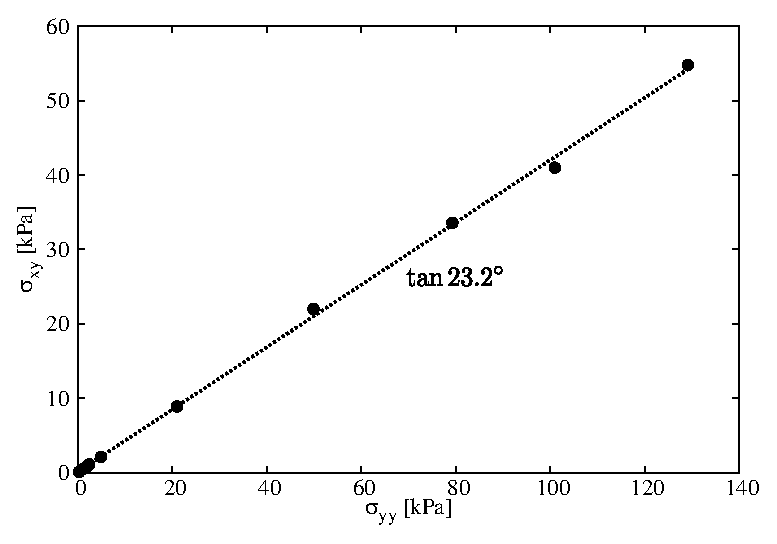
\includegraphics[width=\textwidth]{Sxy_vs_Syy}
\caption{Critical state friction angle from periodic shear test}
\label{fig:Sxy_vs_Syy}
\end{subfigure} 
\caption{Periodic shear test}
\label{fig:shear_test}
\end{figure}

\citet{Guilkey2003} suggests using at least four material points per cell for 
large deformation problems. In the present study, 16 material points 
per cell is adopted. If the mesh is too fine and the number of particles is too 
large, the particle size $2lp$ decreases, and the GIMPM interpolation 
function 
tends to approach the original MPM function, as shown 
by~\citet{Bardenhagen2004}. Hence GIMPM loses the merit that it reduces the 
numerical noise due to material points crossing the background mesh. In 
addition, the probability of particles crossing the background mesh increases 
with decrease in mesh size, hence, more noise can be produced~\cite{Abe2013}. 
The effect of number of material points per cell on the run-out behaviour is 
discussed in~\cref{sec:MPM_points_per_cell}. Each material point represents 
one-fourth of a DEM soil grain. The parameters used for the continuum analyses 
are presented in~\cref{table:MPMData}. 

\begin{table}
\caption{Parameters used in continuum simulations}
\label{table:MPMData}
\centering
\begin{tabular}{ll}
\toprule
\textbf{Parameter} & \textbf{Value} \\ \midrule
Material point spacing & 0.575 \si{\mm} \\
Number of material points per cell & 16 \\
Young's Modulus, E & $1.98 \times 10 ^{6}$ \si{\Pa} \\
Poisson's ratio, $\nu$ & 0.22 to 0.24 \\ 
Friction angle, $\phi$ & $23.2 \pm 0.2\si{\degree}$ \\
Dilatancy angle, $\varPhi$ & $0$\si{\degree} \\
Density, $\rho$ & 1800 \si{\kg\per\m\cubed}\\
Wall friction & 0.466 \\
Time step increment & $1.0 \times 10^{-6}$ \si{\second}\\ \bottomrule
\end{tabular}
\end{table}

\subsection{Deposit morphology}
MPM and DEM simulations of granular column collapse are 
performed by varying the initial aspect ratio of the column. 
The normalized final run-out distance, $\Delta L = 
(L_{\textit{f}}-L_{\textit{0}})/L_{\textit{0}}$, as a function of the initial 
aspect 
ratio `a' of the column is presented in~\cref{fig:run-out}. Similar to the 
experimental 
behaviour a power law relation between the run-out and the initial aspect ratio 
of the 
column is observed. Two distinct flow regimes can 
be seen: (a) for `a' <1.7 a linear relation between the spread and aspect ratio 
can 
be observed, and (b) for `a' > 1.7 a power-law relationship exists. In the 
present study, 
the following scaling law for the run-out (using DEM) is observed:
\begin{align}
\frac{L_{\textit{f}}-L_{\textit{0}}}{L_{\textit{0}}} \approx  
\begin{cases}
1.67 a, &\qquad \textit{a}\lesssim 2.3 \\
2.5 a^{2/3}, &\qquad \textit{a} \gtrsim 2.3 \\
\end{cases}
\end{align}
Both, MPM and DEM simulations are able to capture the linear relationship for 
`a' < 1.7, and the simulation results agree with the experimental 
investigation~\cite{Lajeunesse2005}. This shows that a simple frictional 
dissipation model is able to capture the flow dynamics for columns with smaller 
aspect ratio. For `a' < 1.7, the normalised run-out distance predicted using 
DEM simulations are very close to the run-out observed in the experiments. DEM 
simulations with hexagonal packing shows shorter run-out distances in 
comparison to randomly packed sample. This difference in the run-out behaviour 
might be due to the crystallisation and jamming effects in hexagonal packing. 
The small difference in the final run-out between DEM and experimental results 
can be attributed to the variation in the packing of grains. Also, the 
experimental data corresponds to granular column collapse in a rectangular 
channel, the collapse is not a pure two-dimensional collapse as in the case 
of numerical simulations. 

Significant difference in the final run-out between MPM, which is based on a 
simple frictional model for dissipation of potential energy, and DEM 
simulations for `a' > 1.7 indicates a change in the mechanism of energy 
dissipation for columns with large aspect ratios (`a' > 
1.7).~\cite{Staron2005b} observed that a constant frictional dissipation 
model cannot describe a power-law relation observed at large aspect ratio. A 
transition in the run-out behaviour at an aspect ratio of 1.7 indicates a 
change in flow dynamics. Similar behaviour in the run-out distance was observed 
by~\citet{Bandara2013} for columns with large the aspect ratio $\ge 2$.

The longer run-out distance in MPM simulations at large aspect ratios might be 
influenced by the amount of material mobilised during the collapse. In tall 
columns, the entire column participates in the flow, in contrast to short 
columns where the collapse is due to avalanching of 
flanks,~\citet{Lajeunesse2004}. It is possible that MPM simulations 
collapses more resulting in longer run-out distance.~\Cref{fig:height} shows 
the normalized final height as a function of the initial aspect ratio of the 
column. Similar to the run-out behaviour, the normalised-height also shows two 
distinct regimes. The scaling of final height of the column with the initial 
aspect ratio of the column can be written as
\begin{align}
\frac{H_{\textit{f}}}{L_{\textit{i}}} \propto  
\begin{cases}
\textit{a}, \qquad & \textit{a}\lesssim0.7 \\
\textit{a}^{2/3}, \qquad & \textit{a}\gtrsim0.7 \\
\end{cases}
\end{align} 

The final height predicted by both DEM and MPM simulations match the 
experimental data for columns with smaller aspect ratio ($`a' \le 0.7$). Linear 
relationship between the final height and the aspect ratio indicates that only 
a part of the granular column is mobilised during the collapse. For tall 
columns, both approaches predict similar normalised height. However, the 
normalised height observed in MPM is higher than in DEM simulations, which is 
in contrast to the idea of increase in the amount of material mobilised during 
the collapse in MPM simulations resulting in longer run-out distance. Hence, 
the longer run-out observed in MPM simulations is due a change in the 
flow dynamics at higher aspect ratios, which is not captured in MPM 
simulations. The final height of a column is controlled by the amount of static 
region in the granular column collapse, while the run-out distance is 
essentially a function of the flowing mass. Hence, it is essential to compare 
the evolution of flow and the internal flow structure in DEM and MPM 
simulations.

\begin{figure}[tbhp]
\centering
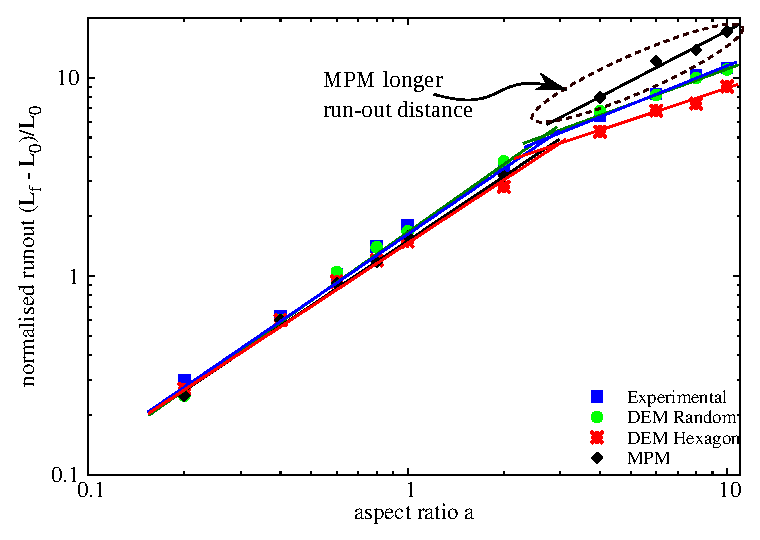
\includegraphics[width=\textwidth]{runout}
\caption{Normalised final run-out distance for columns with different initial 
aspect ratio}
\label{fig:run-out}
\end{figure}

\begin{figure}[tbhp]
\centering
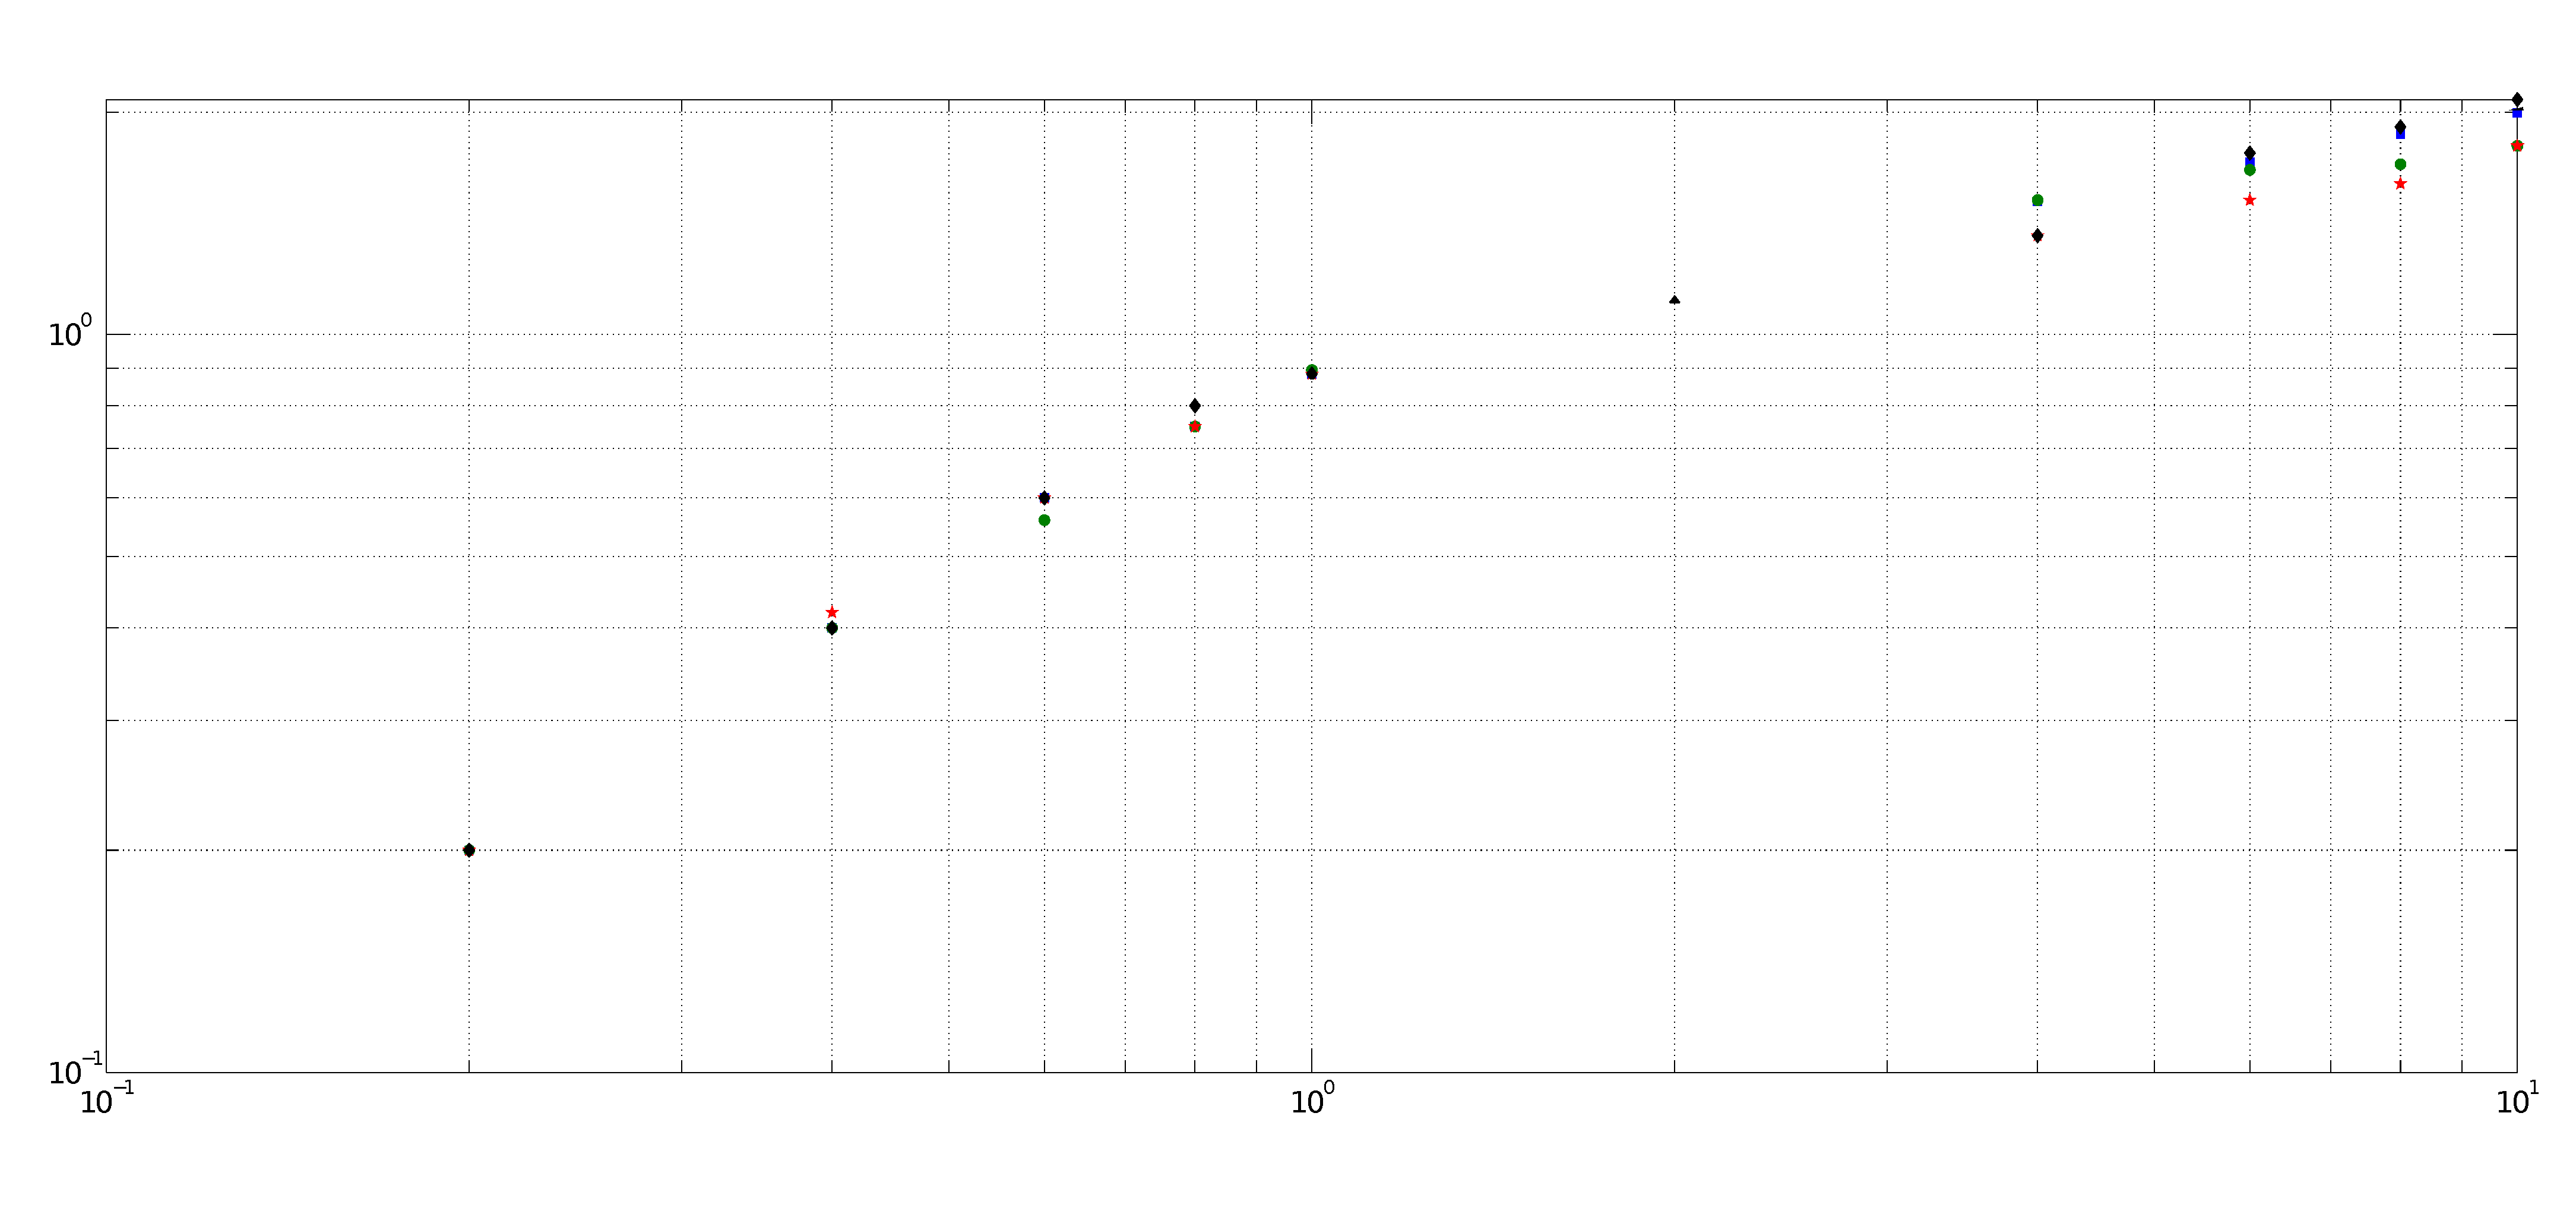
\includegraphics[width=\textwidth]{height}
\caption{Normalised final collapse height for columns with different initial 
aspect ratio}
\label{fig:height}
\end{figure}

\subsection{Flow evolution and internal flow structure}

The normalised run-out and height as a function of the aspect ratio indicates 
that, for a given granular material and substrate properties, the flow dynamics 
and the final deposit morphology are independent of the volume of granular 
material released, but depend only on the geometry of the column. A 
power law relationship is observed between the run-out distance and the initial 
aspect ratio of the column. A transition in the run-out behaviour at an aspect 
ratio of 2.3 indicates a change in the flow dynamics. 

For smaller aspect columns (`a' < 2.3), the flow is initiated 
by a failure at the edge of the pile along a well-defined fracture surface.
The granular mass fails through avalanching of flanks producing a 
truncated cone-like deposit (`\textit{a}' < 0.7) or conical deposit 
(`\textit{a}' > 0.7). The grains located above the failure surface move 
``\textit{en masse}'' leaving a static region underneath the failure surface. 

Dimensional analysis of granular column collapse reveals an intrinsic time 
defined as $\sqrt{H_{\textit{i}}/g}$. This intrinsic time is a transient time 
of order $\tau_{c}$, at which the flow is fully developed, i.e., the potential 
energy available at the initiation of collapse is now fully converted to 
kinetic energy. Numerical simulation of the velocity profile of a granular 
column (`a'=0.4) at critical time $\tau_{c}$ is presented in \cref{fig:a04tc}. 
At critical time, the velocity field depends only on the position of the grain 
along the sliding mass. The maximum velocity is observed at the front of the 
flowing mass corresponding to that of a plug flow in horizontal direction. 
Particulate and continuum simulations show similar run-out distance at the 
critical time. Both approaches show similar quantity of material destabilised 
above the failure surface. However, the crystalline arrangement of soil grains 
in a hexagonal packing results in a different flow mechanics, which also 
shows the effect of jamming at the flow front. The continuum nature of MPM 
results in a slightly different geometry of the material destabilised above the 
failure surface in comparison to DEM simulations. The velocity profile is 
similar to a steady granular surface flow observed by~\citet{Lajeunesse2004}. 

For columns with lower initial aspect ratios, the run-out distance is 
proportional to the mass flowing above the failure surface. The spreading 
results from a Coulomb-like failure of the edges and implies no free fall of 
the column. ~\citet{Daerr1999} also observed active Coulomb yielding in 
transient granular surface flows. In this case, the effective friction 
properties of the flow can be simply predicted from the shape of the final 
deposit. The amount of mass mobilized during the collapse is significantly 
affected by the angle of the failure surface.~\Cref{fig:a04tc} shows that both 
numerical techniques predict a distinct failure surface when the flow is fully 
developed at critical time $\tau_{\textit{c}}$. The angle of the failure 
surface is found to be about $55^{o}$. The failure surface begins from the toe 
of the column and protrudes inwards at an angle of $50$ to 
$55\si{\degree}$. The formation of the ``truncated conical deposit'' or 
``conical deposit'' depends only on the initial length of the column, as the 
angle of the failure surface is found to be independent of the aspect ratio. 
The failure angle is consistent with the interpretation in terms of 
\textit{active Coulomb failure}~\citep{Lajeunesse2004}, which leads to a 
predicted failure angle $\theta_{\textit{y}}=45\si{\degree}+\delta / 2$, where 
$\delta$ is the internal friction angle of the granular material. In the 
present study, the friction angle of the glass beads is $22\si{\degree}$, which 
leads to $\theta_{\textit{y}}=45\si{\degree}+22\si{\degree}/ 2=56\si{\degree}$, 
which is in good agreement with the numerical simulations and experimental 
observations by~\citet{Lajeunesse2004}. The fracture angle has a 
direct effect on the transition between the truncated cone and the conical 
deposit occurring at an aspect ratio of 0.7.~\citet{Schaeffer1990} observed the 
onset of instabilities in a narrow wedges of $56\mbox{ to }65^{o}$ for 
Cambridge-type constitutive models that describes granular flows, which is 
in-line with the failure angle observed in the present study. 

The final profile of the granular column with an initial aspect ratio 
of 0.4 is shown in \cref{fig:a04f}. Both MPM and DEM show similar run-out 
behaviour. The continuum approach is able to capture the flow dynamics of short 
columns, wher the failure mechanism is active Coulomb failure. In dense 
hexagonal packing, the failure surface is steep due to crystallisation effect. 
The variation in the angle of the failure surface causes a difference in the 
amount of material destabilised, and in turn in the run-out distance. 
This crystallisation phenomenon is found to have a significant influence on the 
final deposit of the granular column.~\citet{Lacaze2009} observed that 
poly-disperse grains have lesser tendency to crystallize especially in the case 
of tall columns. 

\begin{figure}[tbhp]
\centering
\includegraphics[width=\textwidth]{a04tc}
\caption{Velocity profile of a granular column collapse ($`a' = 0.4$ \& 
$t=\tau_c$)}
\label{fig:a04tc}
\end{figure}

\begin{figure}[tbhp]
\centering
\includegraphics[width=\textwidth]{a04f}
\caption{Velocity profile of a granular column collapse ($`a' = 0.4$ \& 
$t=3\times\tau_c$)}
\label{fig:a04f}
\end{figure}


For tall columns (`a' > 2.3), the flow is still initiated by a well defined 
failure surface as can be seen in~\cref{fig:a6tc}. However, in this case the 
initial granular column is much higher than the top of the failure surface. Due 
to gravity most of the grains in the column experience free-fall 
consuming the column along their way. When they reach the vicinity of the 
failure surface, the flow gets deviated along the horizontal direction 
releasing a huge amount of kinetic energy gained during the free fall. For 
larger aspect ratio (\textit{a} > 0.7), the resulting static region is a cone, 
the final height of the cone, i.e, $\textit{H}_{\textit{f}}$ lies above the 
summit of the failure surface. Hence, a different evolution is observed from 
that of the axis-symmetric geometry~\citep{Lube2005}, where the final height 
coincides with the summit of the failure surface forming a truncated conical 
deposit.~\citet{Lajeunesse2004} observed that the variation in the deposit 
morphology between the axis-symmetric case and the rectangular collapse to be a 
geometrical effect rather than as an experimental artefact. 

An initial failure surface starting from the toe end 
of the column at an angle of about 55$^{o}$ can be observed at the critical 
time $\tau_{c}$. As the collapse of the granular collapse progresses, 
successive failure planes parallel to the initial failure surface are formed 
and shear failure occurs along these planes. The presence of several shear 
bands in the final profile of the collapsed granular column confirms this 
hypothesis. Crystallisation in hexagonal packing has a significant effect on 
the run-out distance by forming series of parallel shear bands, resulting in 
unnatural flow kinematics. However, MPM exhibits a single failure surface. This 
observation throws light on 
the mechanics of propagation of shear bands in massive landslides such as the 
Storegga submarine landslide. The flow behaviour becomes similar to that of 
columns with lower aspect ratio as the flow starts descending along the failure 
plane. The final profile of the collapsed granular column with an initial 
aspect ratio of 6 is presented in Figure.\ref{fig:a6f}. For tall columns, the 
dissipation process is more complex due to the free-fall dynamics. The vertical 
acceleration of the grains induces a non-trivial mass distribution in the flow 
while spreading. This mass distribution plays a dominant role in the power-law 
scaling law obeyed by the run-out~\citep{Staron2007}.

Regardless of the experimental configuration and the initial aspect ratio of 
the columns, the flow is initiated by a well-defined rupture surface, above 
which the material slides down leaving a static region underneath the failure 
plane. Depending on the aspect ratio of the column, two asymptotic behaviours 
are observed. For smaller aspect ratios, the flow is dominated by friction 
where as large aspect ratio columns are influenced by the pressure gradient.

\begin{figure}[tbhp]
\centering
\includegraphics[width=\textwidth]{a6tc}
\caption{Velocity profile of a granular column collapse ($`a' = 6$ \& 
$t=\tau_c$)}
\label{fig:a6tc}
\end{figure}

\begin{figure}[tbhp]
\centering
\includegraphics[width=\textwidth]{a6f}
\caption{Velocity profile of a granular column collapse ($`a' = 6$ \& 
$t=3\times\tau_c$)}
\label{fig:a6f}
\end{figure}

To study the influence of aspect ratio on the flow dynamics of granular 
columns, the flow front \textit{L}(\textit{t}) and the maximum height of column 
\textit{H}(\textit{t}) are tracked. The evolution of scaled height 
$(H_{\textit{f}}/L_{\textit{0}})$ and the run-out distance 
$(L_{\textit{f}}-L_{\textit{0}})/L_{\textit{0}}$ with time for granular columns 
with an initial aspect ratio of 0.4 and 6 are presented in
~\cref{fig:flow_column}. Three distinct regions can be observed in the flow 
evolution of a granular column collapse regardless of the initial aspect ratio 
of the column. An initial transient acceleration phase is observed for a time 
0.8$\tau_{c}$. 
This phase is followed by a heap movement of granular materials at the foot 
with a constant spreading velocity \textit{V} for about 2$\tau_{c}$. When time 
`\textit{t}' $> \tau_{c}$, the velocity varies linearly with depth in the 
flowing layer and decreases exponentially with depth near the static layer. 
This velocity profile is similar to those observed in steady granular surface 
flows~\citep{Lajeunesse2004}. Most of the run-out happens during this phase. 
The final phase involves deceleration of the flow front and the flow comes to 
rest after about 0.6$\tau_{c}$. The spreading of the granular column ceases 
after a time in the order of about 3$\tau_{c}$, however some motion still 
persists along the free surface behind the flow front for a much longer time 
due to internal rearrangement, the duration of which can last up to $\textit{t} 
\approx 6\tau_{c}$. 

The critical time is evaluated as the time at which the potential energy 
available for the flow has been converted to the kinetic energy. In short 
columns, the critical time observed in both hexagonal and random packing of 
grains matches the experimental observations. However, the Material Point 
Method overestimates the critical time by a factor of 1.25, which means that it 
takes longer for the flow to be fully mobilized. However, the actual run-out 
duration of the flow is short and the granular mass comes to rest at about 
$\textit{t}=3\tau_{c}$.
 
For columns with larger aspect ratios, the continuum and particulate approaches 
simulate similar flow evolution behaviour for times up to 3$\tau_{c}$, beyond 
which particulate simulation decelerates and comes to rest, while the flow 
continues to evolve in MPM simulations resulting in longer run-out distance. 
The flow comes to rest at time $\textit{t}=6\tau_{c}$. The 
three phases in a granular flow can be distinctly observed in the flow 
evolution plot for a granular column with initial aspect ratio of 6 (see 
~\cref{fig:flowa6}). The flow evolution 
behaviour observed in the case of DEM simulation matches the experimental 
observation by~\citet{Lajeunesse2004}. Hexagonal packing predicts longer time 
for the flow to evolve, which can be attributed to crystallisation of grains. 
In MPM simulations, the failure starts at the toe of the column and slowly 
propagates up to form the failure surface. This results in slower initiation of 
the flow. It can be observed that MPM overestimates the critical time by 50\%. 
Although, MPM and DEM simulations show the same run-out at time 
$\textit{t}=3\tau_{c}$, the flow evolution between both the approaches is 
different. MPM simulations continue to accelerate beyond $3\tau_c$ and ceases 
to flow at $6\tau_{c}$. In order to understand the difference in the flow 
dynamics in the case of Material Point Method it is important to study the 
mechanism of energy dissipation. 


\begin{figure}[tbhp]
\centering
\begin{subfigure}[b]{0.975\textwidth}
\centering
\includegraphics[width=\textwidth]{flowa04}
\caption{Flow evolution of a column with $`a'=0.4$}
\label{fig:flowa04}
\end{subfigure}
\\
\begin{subfigure}[b]{0.975\textwidth}
\centering
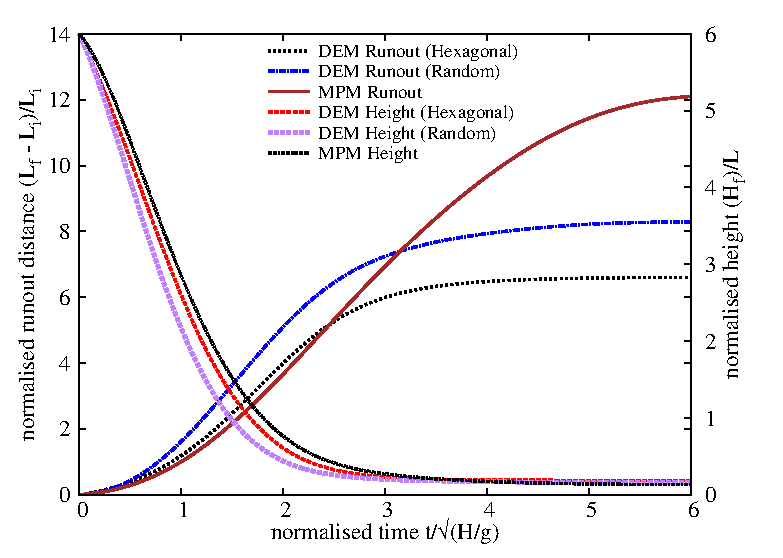
\includegraphics[width=\textwidth]{flowa6}
\caption{Flow evolution of a column with $`a'=6$}
\label{fig:flowa6}
\end{subfigure}
\caption{Flow evolution of granular column collapse}
\label{fig:flow_column}
\end{figure}

\subsection{Energy dissipation mechanism}
\label{sec:energy}

The energy dissipation mechanism during the collapse provides useful insight 
into the flow dynamics. In the case of small aspect ratios, the columns undergo 
no free fall. The spreading mainly results from the failure of the edges, while 
the top of the column remains essentially undisturbed in the central area. 
~\citet{Staron2007} showed that the amount of energy dissipated during the 
spreading $\delta E$ can be easily recovered using the simple shape of the 
final deposit and volume conservation (see~\cref{fig:volume_conservation}). The 
difference of potential energy between the initial and the final states gives

\begin{equation}
\delta E = \frac{1}{6} g \rho (L_f - L_0) H_0^2 \,,
\end{equation}

\begin{figure}
\centering
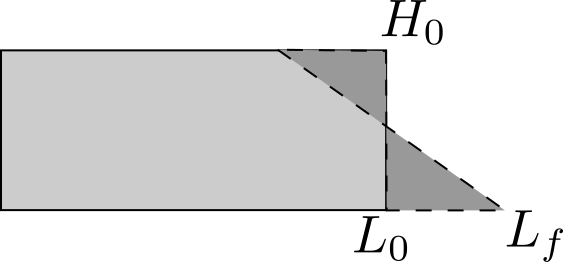
\includegraphics[width=0.7\textwidth]{volume_conservation}
\caption{Scheme of collapse for small aspect ratio columns. The amount of 
energy $\delta E$ lost in the process can be evaluated
from the run-out distance $L_f - L_0$ (after~\citet{Staron2007}).}
\label{fig:volume_conservation}
\end{figure}

where $\rho$ is the density of the packing. It is assumed that this energy is 
dissipated by the work of friction forces $W_{\mu}$ over the total distance run 
by the center of mass G of the spreading material.~\citet{Staron2006} considers 
two regions of dissipation: the amount of mass destabilised $\frac{1}{4}(L_f - 
L_0) H_0$ over two thirds of the runout distance $2(L_f - L_0) / 3$ (considering
the triangular shape of the final deposit and the initial and final positions 
of the center of mass). The effective coefficient of friction $\mu_e$ 
characterizes he mean dissipation in the flow. The work of friction forces is 

\begin{equation}
W_{\mu} = \frac{1}{6} \mu_e g \rho (L_f - L_0) H_0^2 \,,
\end{equation}

Equating $\delta_E$ and $W_{\mu}$ gives $\mu_e (L_f - L_0) = H_0$. The scaling
of the runout leads directly to the relation $\mu_e = \lambda^-1$, which is the 
numerical constant in the power law of the run-out that depends on the material 
properties~\citep{Balmforth2005}. The amount of energy $\delta E$ dissipated 
during the spreading is compared with $W = N_p g m_p r_p$, where $N_p$ is the 
total number of grains, $m_p$ is their mass, and $r_p$ is the total horizontal 
distance run by each of them. We observe that the dissipation energy $\delta E$ 
is proportional to $W$.~\cite{Staron2007} observed that the coefficient of 
proportionality gives a measure of the effective friction and 
observed a power law dependence between $\mu_e$ and internal friction angle 
$\mu$: $\mu_e=0.425\mu^{0.2}$. The effective friction angle $\mu_e$ of 
21\si{\degree} is observed, which is very close to the critical state friction 
angle of 22\si{\degree} used in MPM simulations. This proves that the energy 
dissipation mechanism modelled in a continuum sense as a frictional dissipation 
process captures the flow kinematics observed in DEM and experiments, for short 
columns.

~\Cref{a04_energy} shows the time evolution of the normalised potential energy 
$(E_{p}/E_0)$ and kinetic energy $(E_{k}/E_0)$ for granular columns with 
initial aspect ration `a' = 0.4. The normalised potential and kinetic energy 
are computed as
%
\begin{align}
E_p & = \sum\limits_{p=1}^{N_p}{m_p g h_p} \\
E_{ki} & = \frac{1}{2}\sum\limits_{p=1}^{N_p}{m_p v_p^2}
\end{align}
%
where $N_p$ is the total number of particles, $m_p$ is 
the mass of a particle `\textit{p}', $h_p$ is the height and 
$v_p$ is the velocity of the particle `\textit{p}'. The cumulative dissipation 
energy is computed as
%
\begin{align}
\frac{E_d}{E_0} = 1 - \frac{E_k}{E_0} - \frac{E_p}{E_0} \,.
\end{align}
%
It can be observed that both MPM and DEM show similar energy dissipation 
mechanism. The DEM simulation shows 3\% more potential energy dissipation in 
comparison with MPM simulations. This small difference in the potential energy 
is due to grain rearrangements. This shows the ability of continuum approach in 
capturing the flow kinematics of columns with small aspect ratios ($`a' \le 
2.3$). 

 
The evolution of normalised kinetic and potential energy of a tall column 
collapse (`a' of 6) is shown in~\cref{fig:a6_energy}. It can be 
observed from the figure that the initial potential energy stored in the 
particle is converted to kinetic energy which is dissipated as the granular 
material flows down. Three successive stages can be identified in the granular 
column collapse. The flow is still initiated by a well defined failure surface. 
However, the centre of gravity of the granular column is much higher than the 
top of the failure surface, which results in free fall of grains under gravity 
consuming the column along their way. In this stage 
$(t<0.8\tau_{c})$, the initial potential energy stored in the grains is 
converted into vertical motion. In the second stage, when the grains reach the 
vicinity of the failure surface, they undergo collisions with the bottom plane 
and the neighbouring grains, thus causing the flow to deviate along the 
horizontal direction releasing a large amount of kinetic energy gained during 
the free fall (see~\cref{fig:a6f}). In the third stage, the grains eventually 
leave the base area of the column and flow sideways~\citep{Lajeunesse2004}. As 
the process involves collective dynamics of all the grains, it is difficult 
to predict the exact trajectory of a grain, however, the overall dynamics can 
be explained. 


DEM simulations model both collisional and frictional dissipation process 
during the collapse of tall columns. However, MPM simulations assume that the 
total initial potential energy stored in the system is completely dissipated 
through friction over the entire run-out distance, this results in longer 
run-out distance.~\Cref{fig:a6_energy} shows the evolution of energy with time. 
At the initial stage of collapse, characterised by free fall of grains under 
gravity, DEM simulation due its particulate nature shows a rapid reduction in 
the potential energy in comparison with MPM, where the failure begins from the 
toe of the column. The continuum nature of MPM simulations results in slower 
initiation of collapse (see~\cref{fig:flowa6}). It can be also observed 
from~\cref{fig:a6_energy} that dissipation energy in MPM is 25\% less than DEM 
simulations. In order to understand the mechanism of energy dissipation, it is 
important to understand the contribution from the cumulative frictional and 
collisional parts. The frictional dissipation (basal and internal friction) 
observed in DEM is almost identical to the frictional dissipation observed in 
MPM. The difference in the dissipation energy is due to the collisional regime, 
which occurs at $0.8\tau_c$. The total and frictional dissipation curves 
diverge around $0.8\tau_c$ where the grains near the vicinity of the failure 
surface undergo collisions with the bottom plane and the neighbouring grains 
resulting in collisional dissipation of the stored potential energy. DEM 
simulation show drop in the peak kinetic energy at $\approx0.8\tau_c$, which is 
at the beginning collisional dissipate stage. MPM lacks this collision 
dissipation mechanism, which results in longer run-out distances for columns 
with large aspect ratios. 

\begin{figure}[tbhp]
\centering
\begin{subfigure}[b]{0.975\textwidth}
\includegraphics[width=\textwidth]{a04_energy}
\caption{Energy evolution of a column with $`a'=0.4$}
\label{fig:a04_energy}
\end{subfigure}
\\
\begin{subfigure}[b]{0.975\textwidth}
\centering
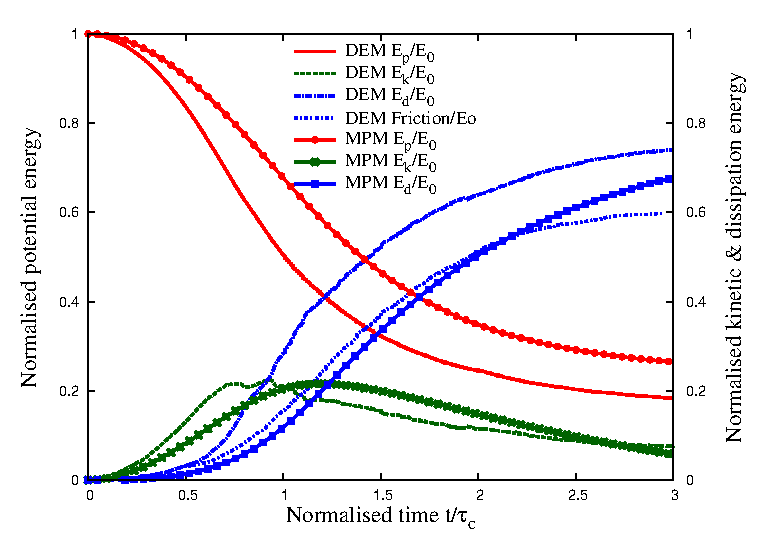
\includegraphics[width=\textwidth]{a6_energy}
\caption{Energy evolution of a column with $`a'=6$}
\label{fig:a6_energy}
\end{subfigure}
\caption{Energy evolution of granular column collapse}
\label{fig:column_energy}
\end{figure}

$\mu(I)$ rheology, discussed in~\cref{sec:muI}, describes the granular 
behaviour using a dimensionless number, called the \textit{inertial number I}, 
which is the ratio of inertia to pressure forces. Small values of I 
corresponds to critical state of soil mechanics and large values of I 
corresponds to the fully collisional regime of kinetic theory. $\mu(I)$ 
rheology is adopted in MPM simulations to understand the characteristics of the 
flow regime. Mohr-Coulomb model was used along with $\mu(I)$ rheology. Friction 
angle is changed according to the value obtained by~\citet{DaCruz2005} friction 
law that is dependent on the inertial number \textit{I} as $\mu = \mu_{min} + b 
\mathit{I}$ where $\mu_{min} = 0.22$ and b = 1.~\Cref{fig:flow_muI} shows the 
flow evolution of granular column collapse for aspect ratio `a' of 0.4 and 6 
using $\mu(I)$ rheology. For short columns, the evolution of flow based on 
$\mu(I)$ rheology is identical to the MPM simulation using Mohr-Coloumb model. 
However, for tall columns, $\mu(I)$ rheology evolves at the same rate as the 
DEM simulations up to $t = 0.8\tau_c$, after which MPM simulation continues to 
accelerate due to lack of collisional dissipation, while the DEM simulation 
decelerates with time. 

\begin{figure}[tbhp]
\centering
\begin{subfigure}[b]{0.975\textwidth}
\includegraphics[width=\textwidth]{flowa04muI}
\caption{Flow evolution of a column with $`a'=0.4$ using $\mu(I)$ rheology}
\label{fig:flowa04muI}
\end{subfigure}
\\
\begin{subfigure}[b]{0.975\textwidth}
\centering
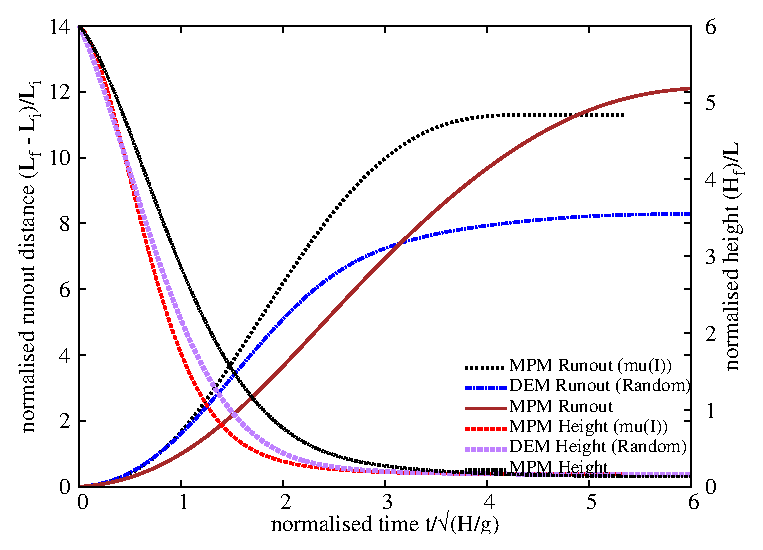
\includegraphics[width=\textwidth]{flowa6muI}
\caption{Flow evolution of a column with $`a'=6$ using $\mu(I)$ rheology}
\label{fig:flowa6muI}
\end{subfigure}
\caption{Flow evolution of granular column collapse using $\mu(I)$ rheology}
\label{fig:flow_muI}
\end{figure}

~\Cref{fig:mu_vs_I} shows that the short column attains a maximum inertial 
number of 0.012, which is in the dense granular flow regime, inertial number 
\textit{I}$\approx10^{-3}$ to $0.1$~\citep{DaCruz2005}. However, the maximum 
inertial number $I\approx0.04$, for tall is still within the 
dense granular flow regime. DEM simulations, however, showed a collisional 
regime that has inertial number higher than 0.1. This shows that continuum 
approach using frictional laws are able to capture the flow kinematics at small 
aspect ratios, however are unable to precisely describe the flow behaviour for 
tall columns, which is characterised by an initial collisional regime.

\begin{figure}[tbhp]
\centering
\includegraphics[width=\textwidth]{muI}
\caption{Evolution of inertial number with time for columns with $`a'=0.4$ and 
$`a'=6$}
\label{fig:muI}
\end{figure}

\subsection{Role of initial grain properties}

\citet{Lube2005} observed that the run-out distance scales with the initial 
aspect ratio of the column, independent of the material properties. The 
run-out 
evolution after the initial transition regime is a frictional dissipation 
process, and the lack of influence of material properties on the run-out 
behaviour is inconsistent with continuum modelling of granular flow behaviour. 
~\citet{Balmforth2005} observed that the material properties have almost no 
influence on the exponent of the normalised run-out as a function of the 
initial aspect ratio. The numerical constant of proportionality, however, 
showed clear material dependence. This corroborates the conclusions 
of~\citet{Lajeunesse2004} and softens that 
of~\citet{Lube2005}.~\citet{Daerr1999} also observed strong influence of 
initial packing density and the internal structure on the behaviour of 
granular 
flows. 


It should be noted that the collapse experiment is highly transient and no 
clear stationary regime is observed. On the contrary, the acceleration and the 
deceleration phases cover nearly the whole duration of the spreading. This 
makes it difficult to analyse the flow structure and its relation with other 
characteristic of the system. The knowledge of the final run-out is not a 
sufficient characterization of the deposit: one also needs to know how the mass 
is distributed during the flow to understand the dynamics and the dissipation 
process. This is expected to be true in natural contexts as well as in 
experiments. While the inter-grain friction does not affect the early vertical 
dynamics, nor the power-law dependence,it controls the effective frictional 
properties of the flow, and its internal structure~\citep{Staron2007}. It is 
interesting to note that the details of the structure of the flow do not 
influence the final run-out dependence, and thus seem to play a marginal role 
in the overall behaviour of the spreading. This could explain why simple 
continuum model with a frictional dissipation could reproduce the run-out 
scaling for columns with small aspect ratios.

The run-out behaviour of a loose (79\% packing fraction) and a dense (83\% 
packing) granular column (a = 0.8) is studied to understand the influence of 
material properties. The evolution of normalised run-out with time for two 
different initial packing 
densities are presented in~\cref{fig:runout_height_dense_r18}. At the initial 
stage of collapse $t=\tau_c$, the flow behaviour is identical in both dense and 
loose conditions. However, the dense column flows 30\% longer than the loose 
condition. Both the columns come to rest at around $t = 4\tau_c$. The columns, 
however, show similar evolution of the normalised height. This shows that only 
a part of the column is destabilised during the collapse.
\begin{figure}[h]
\centering
\includegraphics[width=0.9\textwidth]{runout_height_dense_r18}
\caption{Effect of density on run-out evolution $`a' = 0.8$}
\label{fig:runout_height_dense_r18}
\end{figure}

\begin{figure}[h]
\centering
\includegraphics[width=0.9\textwidth]{voro_r18}
\caption{Evolution of local packing density $`a' = 0.8$}
\label{fig:voro_r18}
\end{figure}

~\Cref{fig:Energy_density_r18} show the evolution of potential and kinetic 
energy with time. Similar potential energy evolution in both dense and loose 
conditions reveals that there is no change in the overall mechanism of 
collapse. The dense condition has slightly higher peak kinetic energy than the 
loose column. In the free-fall phase, the dense column shows a steeper increase 
in the horizontal kinetic energy in comparison with the loose column. This 
indicates that dense granular mass is pushed farther away more quickly than the 
loose column. Loose column exhibits higher vertical kinetic energy which may be 
due to particle rearrangement resulting in densification of the granular 
mass.~\cref{fig:voro_r18} shows that the loose sample densifies as the flow 
evolves. Both dense and loose granular columns dilate during the initial stage 
of collapse, this is due to grains failing by shear along the fracture surface. 
In both cases, the granular mass attains similar packing density at the end of 
the flow. Dense granular column dilates, while the loose column compacts to 
achieve the same critical density.~\citet{Lajeunesse2004} observed that the 
flow comes to rest at around $3\tau_c$, but the grains continue to re-arrange 
until $6\tau_c$, similar behaviour is observed in DEM simulations. The dense 
condition has higher mobilised potential energy at the start of the flow, which 
yields higher horizontal kinetic energy for the flow. A higher proportion of 
kinetic energy is lost during compaction, in comparison to the dense granular 
column. This behaviour in addition to higher mobilised potential results in 
longer run-out distance in dense granular column.  
\begin{figure}[tbhp]
\centering
\begin{subfigure}[b]{0.75\textwidth}
\centering
\includegraphics[width=\textwidth]{Energy_dense_r18}
\caption{Evolution of potential and kinetic energy}
\label{fig:Energy_dense_r18}
\end{subfigure}
\\
\begin{subfigure}[b]{0.75\textwidth}
\centering
\includegraphics[width=\textwidth]{KExy_dense_r18}
\caption{Effect of kinetic energy}
\label{fig:KExy_dense_r18}
\end{subfigure}
\caption{Effect of density on energy evolution $a = 0.8$}
\label{fig:Energy_density_r18}
\end{figure}

In order to remove the effect of crystallisation on the run-out behaviour, a 
highly poly-disperse sample ($r = d_{max}/d_{min} = 6)$ is used. 
The flow kinematics of a dense (relative density $D_r = 74\%$) and a loose 
($D_r = 22\%$) granular column with aspect ratio of 0.8 is studied. Similar to 
the previous case, the dense granular column exhibits longer run-out distance 
(see~\cref{fig:runout_height_dense_r6}. Due to compaction of grains in loose 
condition, almost 20\% of the initial potential energy available for collapse 
is lost in densification due to grain rearrangements in comparison to dense 
condition (see~\cref{fig:Energy_voro_r6}). The compaction of grains in loose 
column and the dilation in dense column results in significantly different flow 
structure, especially at the flow front (~\Cref{fig:density_r6}. As the loose 
column densifies, more granular mass is pushed to the flow front resulting in 
higher vertical effective stress. The loose column exhibits a more parabolic 
final deposit profile in comparison to the dense column, which shows a 
triangular deposit at the front.

\begin{figure}[tbhp]
\centering
\includegraphics[width=0.9\textwidth]{runout_height_dense_r6}
\caption{Effect of density on run-out evolution $`a' = 0.8$ (poly-dispersity 
`r' = 6)}
\label{fig:runout_height_dense_r6}
\end{figure}


\begin{figure}[bhp]
\centering
\begin{subfigure}[b]{\textwidth}
\centering
\includegraphics[width=\textwidth]{dense_a08_r6_final}
\caption{Dense initial packing}
\label{fig:dense_a08_r6_final}
\end{subfigure}
\\
\begin{subfigure}[b]{\textwidth}
\centering
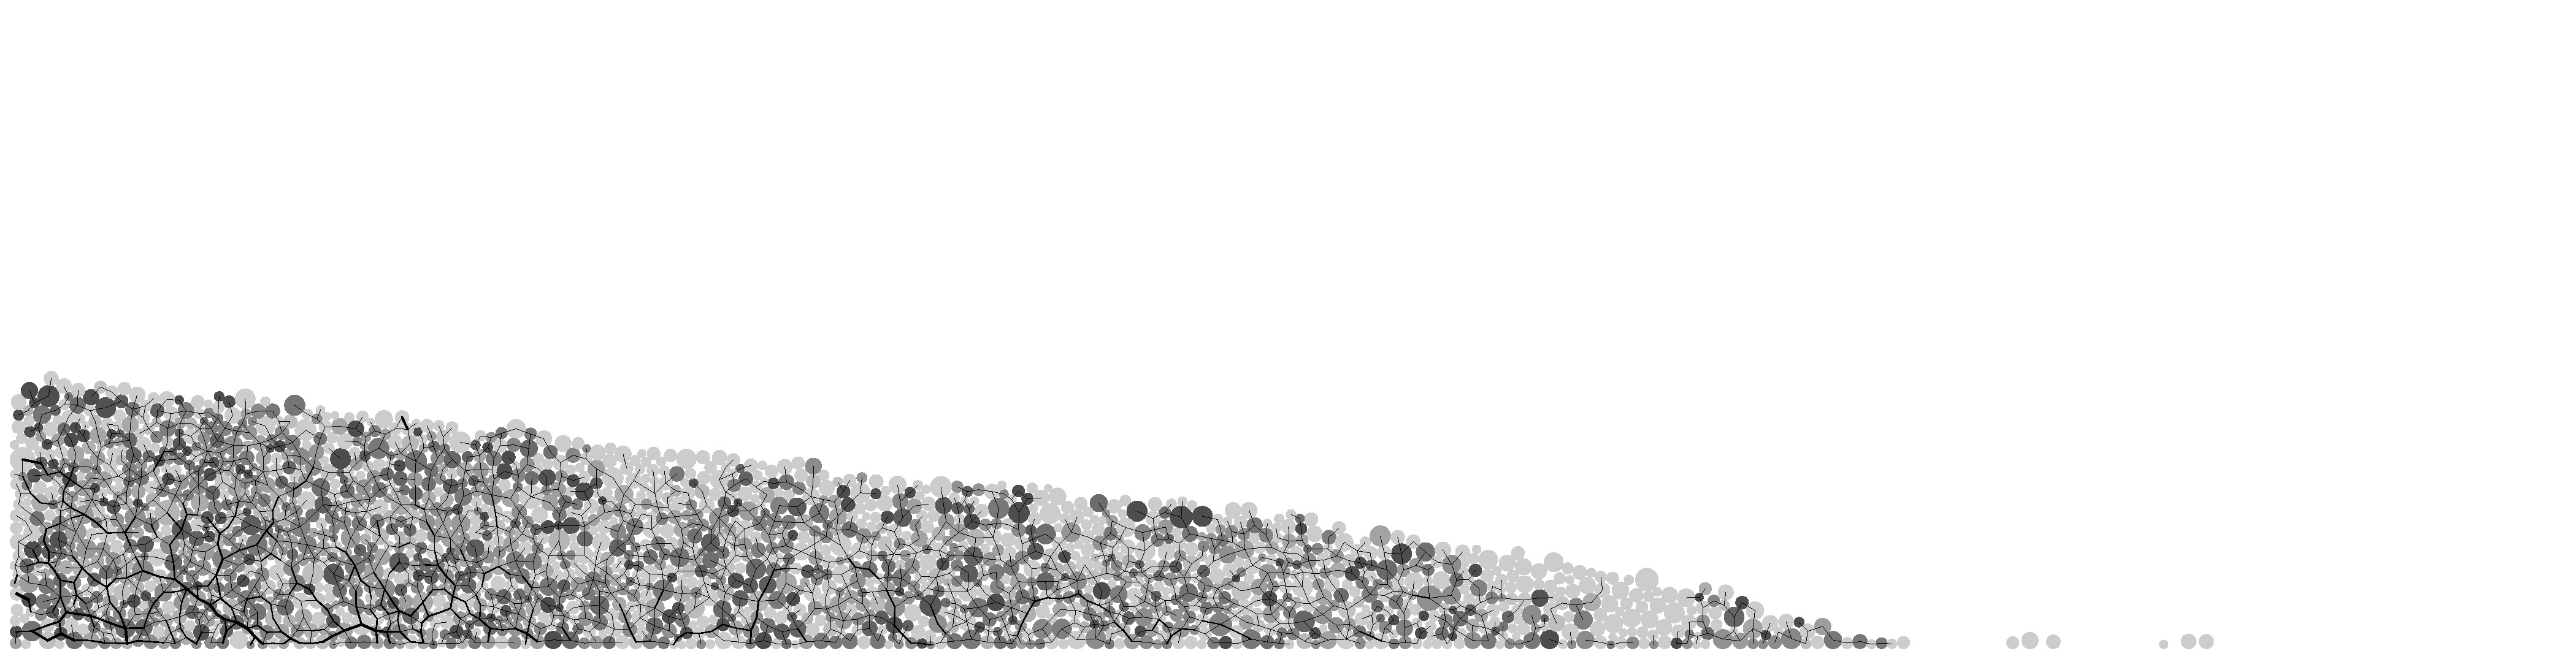
\includegraphics[width=\textwidth]{loose_a08_r6_final}
\caption{Loose initial packing}
\label{fig:loose_a08_r6_final}
\end{subfigure}
\caption{Snapshots of granular column collapse $t = 6 \tau_c$}
\label{fig:density_r6}
\end{figure}


\begin{figure}[tbhp]
\centering
\begin{subfigure}[b]{0.75\textwidth}
\centering
\includegraphics[width=\textwidth]{Energy_dense_r6}
\caption{Evolution of potential and kinetic energy}
\label{fig:Energy_dense_r6}
\end{subfigure}
\\
\begin{subfigure}[b]{0.75\textwidth}
\centering
\includegraphics[width=\textwidth]{voro_r6}
\caption{Evolution of packing density}
\label{fig:voro_r6}
\end{subfigure}
\caption{Effect of density on energy and packing fraction evolution $`a' = 
0.8$ 
(poly-dispersity `r' = 6)}
\label{fig:Energy_voro_r6}
\end{figure}

In short column, only a part of the granular column above the failure surface 
participates in the flow. However, it appears that the collapse for 
large aspect ratios mixes two very different dynamics: while the second stage 
consists of a ``conventional''horizontal granular flows, the first stage 
implies a large vertical acceleration. It shows how the initial condition can 
influence the overall behaviour of a granular system. The effect of density on 
the run-out behaviour of tall columns is investigated. Similar to short 
columns, the dense granular column with aspect ratio of 6 shows higher run-out 
distance in comparison to the loose condition. The dense granular flows almost 
twice as much as that of the loose granular column. Unlike short columns, the 
evolution of run-out is different even at the initial stage of the collapse. 
The dense granular column, which has higher initial potential energy show a 
rapid increase in the run-out due to free-fall and higher mobilised potential 
energy. During the stage of collapse, the dense granular column has 15 \% 
higher normalised kinetic energy available for the horizontal push. This 
results in longer run-out distance for dense granular column in comparison with 
initially loose granular column.

\begin{figure}[tbhp]
\centering
\begin{subfigure}[b]{0.95\textwidth}
\includegraphics[width=\textwidth]{runout_height_dense_a6}
\caption{Effect of density on run-out evolution}
\label{fig:runout_height_dense_a6}
\end{subfigure}
\\
\begin{subfigure}[b]{0.95\textwidth}
\centering
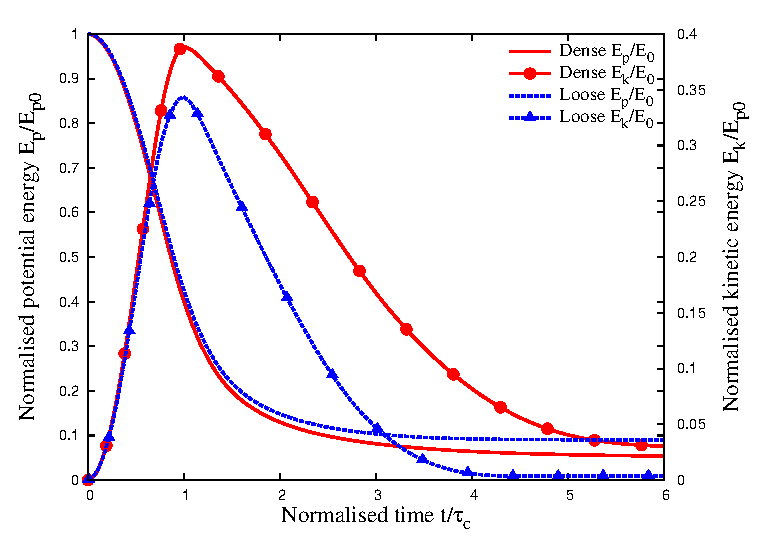
\includegraphics[width=\textwidth]{Energy_dense_a6}
\caption{Effect of density on energy evolution}
\label{fig:Energy_dense_a6}
\end{subfigure}
\caption{Effect of density on run-out behaviour and energy evolution $`a' = 
0.6$}
\label{fig:Density_a6}
\end{figure}

The initial packing fraction has a significant influence on the flow kinematics 
and the run-out behaviour, this suggests that triggering mechanisms play a
crucial role in the case of natural flows. This stresses the necessity of 
accounting for initiation mechanisms while modelling the run-out behaviour 
using continuum approaches to predict realistic granular flow behaviour.

\section{Slopes subjected to impact loading}

Transient granular flows occur very often in nature. Well-known examples are 
rockfalls, debris flows, and aerial and submarine avalanches. In the 
geotechnical context, transient movements of large granular slopes 
is a substantial factor of risk due to their destructive force and the 
transformations they may produce in the landscape. Natural granular flows 
may be triggered as a result of different processes such as gradual 
degradation, induced by weathering or chemical reactions, liquefaction and 
external forces such as earthquakes. Most contemporary research on granular 
materials deals with the steady-state flow. Transients and inhomogeneous 
boundary conditions are much less amenable to observation and analysis, and 
have thus been less extensively studied despite their primary importance in 
engineering practice. In all cases, an initially static pile of grains is 
disturbed by external forces, it then undergoes an abrupt accelerated motion 
and spreads over long distances before relaxing to a new equilibrium state when 
the whole kinetic energy acquired during destabilization is dissipated
by friction and inelastic collisions.

This section investigates the ability of MPM, as a continuum approach, to 
reproduce the evolution of a granular pile destabilized by an external energy 
source. In particular, a central issue is whether power-law dependence of the 
run-out distance and time observed with respect to the initial geometry or 
energy can be reproduced by a simple Mohr-Coulomb plastic behaviour for 
granular slopes subjected an impact energy. Effect of different input 
parameters, such as the distribution of energy and base friction, on the 
run-out kinematics are studied by comparing the data obtained from DEM and MPM 
simulations. As we shall see, MPM is successfully able to simulate the 
transient evolution with a single input parameter, the internal angle of 
friction. This opens the way to the simulation of geological-scale flows on 
complex topographies.

\subsection{Numerical set-up}
\label{sec:num}

The DEM sample 
is composed of $\sim13000$ disks with a uniform distribution of diameters by 
volume fractions ($d_{max} = 1.5 d_{min}$). The mean grain diameter and mass 
are $d\simeq 2.455 $ \si{\mm} and $m\simeq 0.0123$ \si{\kg}, respectively. The 
grains are first poured uniformly into a rectangular box of given width and 
then the right-hand side wall is shifted further to the right to allow the 
grain to spread. A talus is obtained when all grains come to rest; 
see~\cref{fig:slope_configuration}. This procedure leads to a mean packing 
fraction $\simeq 0.82$. Soil grains with mean density of 2600 
\si{\kg\per\m\cubed} and internal friction coefficient of 0.4 between grains 
is adopted.

\begin{figure}[tbph]
\includegraphics[width=0.95\textwidth]{slope_configuration}
\caption{Initial geometry and dimensions of the pile}
\label{fig:slope_configuration}
\end{figure}


The initial static pile is set into motion by applying a constant horizontal
gradient  $v_{0x}(y) = k (y_{max} - y)$ with $k>0$. Such a configuration 
mimics the energy transfer mechanism of a horizontal quake along the bottom of 
the pile. The evolution of pile geometry and the total kinetic energy as a 
function of the initial input energy $E_0$ is studied. The run-out distance 
$L_f$ is the distance of the rightmost grain, which is still in contact with 
the main mass when the pile comes to rest.  The run-out will be normalized by 
the initial length $L_0$ of the pile, as in the experiments of collapsing 
columns. The total run-out duration $t_f$ is the time taken by the pile to 
reach its final run-out distance $L_f$.

For grain scale simulations, classical DEM and Contact Dynamics approach are 
used. This research is done in collaboration with Patrick Mutabaruka, 
University of Montpellier, who performed Contact Dynamics (CD) simulations that 
are 
presented in this section. A detailed description of the Contact Dynamics 
method can be found in \cite{Moreau1993,Jean1999,Radjai2009,Radjai2011}. 
The CD method is based on implicit time integration of the equations of motion 
and a nonsmooth formulation of mutual exclusion and dry friction between 
particles. The CD method requires no elastic repulsive potential and no 
smoothing of the Coulomb friction law for the determination of forces. 
For this reason, the simulations can be performed with large time steps 
compared to discrete element simulations. The unknown variables are particle 
velocities and contact forces, which are calculated at each time step by taking 
into account the conservation of momenta and the constraints due to mutual 
exclusion between particles and the Coulomb friction. An iterative 
research algorithm based on a non-linear Gauss-Seidel scheme is used. The only 
contact 
parameters within the CD method are the friction coefficient $\mu$, the 
normal restitution coefficient $\varepsilon_n$ and the tangential restitution 
coefficient 
$\varepsilon_t$ between particles. 

The natural units of the system are the mean grain diameter $d$, mean grain 
mass $m$ and gravity $g$. For this reason, the length scales are normalised 
by $d$, time by $(d/g)^{1/2}$, velocities by $(gd)^{1/2}$ and energies by 
$mgd$. In MPM simulations the material point spacing is kept the same as the 
mean grain diameter. A mesh size of 0.0125m is adopted with 25 material points 
per cell. The effect of mesh size and the number of material points per cell is 
investigated in~\cref{sec:MPM_points_per_cell}. A Mohr-Coulomb model with no 
dilation is used to simulate the continuum behaviour of the granular pile. 
Periodic shear tests using CD, see~\cref{fig:Sxy_vs_Syy_Slope}, reveals a 
macroscopic friction coefficient of 0.22. The evolution of inertial number with 
friction is presented in~\cref{fig:mu_vs_I}.

\begin{figure}[tbhp]
\centering
\begin{subfigure}[t]{0.475\textwidth}
\includegraphics[width=0.95\textwidth]{Sxy_vs_Syy_Slope}
\caption{Evaluating the critical state friction angle from periodic shear 
test.}
\label{fig:Sxy_vs_Syy_Slope}
\end{subfigure}
%
\begin{subfigure}[t]{0.475\textwidth}
\includegraphics[width=0.95\textwidth]{mu_vs_I}
\caption{Evolution of Inertial number with friction $\mu$}
\label{fig:mu_vs_I}
\end{subfigure}
\caption{Periodic shear test using CD~\citep{Mutabaruka2013}.}
\label{fig:Shear_Test_Slope}
\end{figure}

%-------------------------------------------------------------------------------
\subsection{Evolution of pile geometry and run-out}
\label{sec:evolution}

\Cref{fig:Gradient_Slope_Profile_200J} shows the initial evolution of granular 
slope subjected to an initial impact energy $E_0 = 61$ (in dimensionless units) 
using MPM. As the granular slope is sheared along the bottom, the shear 
propagates to the top leaving a cavity in the vicinity of the left wall. This 
cavity gets partially filled as the granular mass at the top collapse behind 
the flowing mass due to inertia. Similar behaviour is observed during the 
initial stages of the flow evolution using DE and CD techniques
(see~\cref{fig:Gradient_Slope_CD_200J}. Due to inertia, the grains at the top 
of the granular heap roll down to fill the cavity, while the pile continues to 
spread. 

\begin{figure}[tbph]
\centering
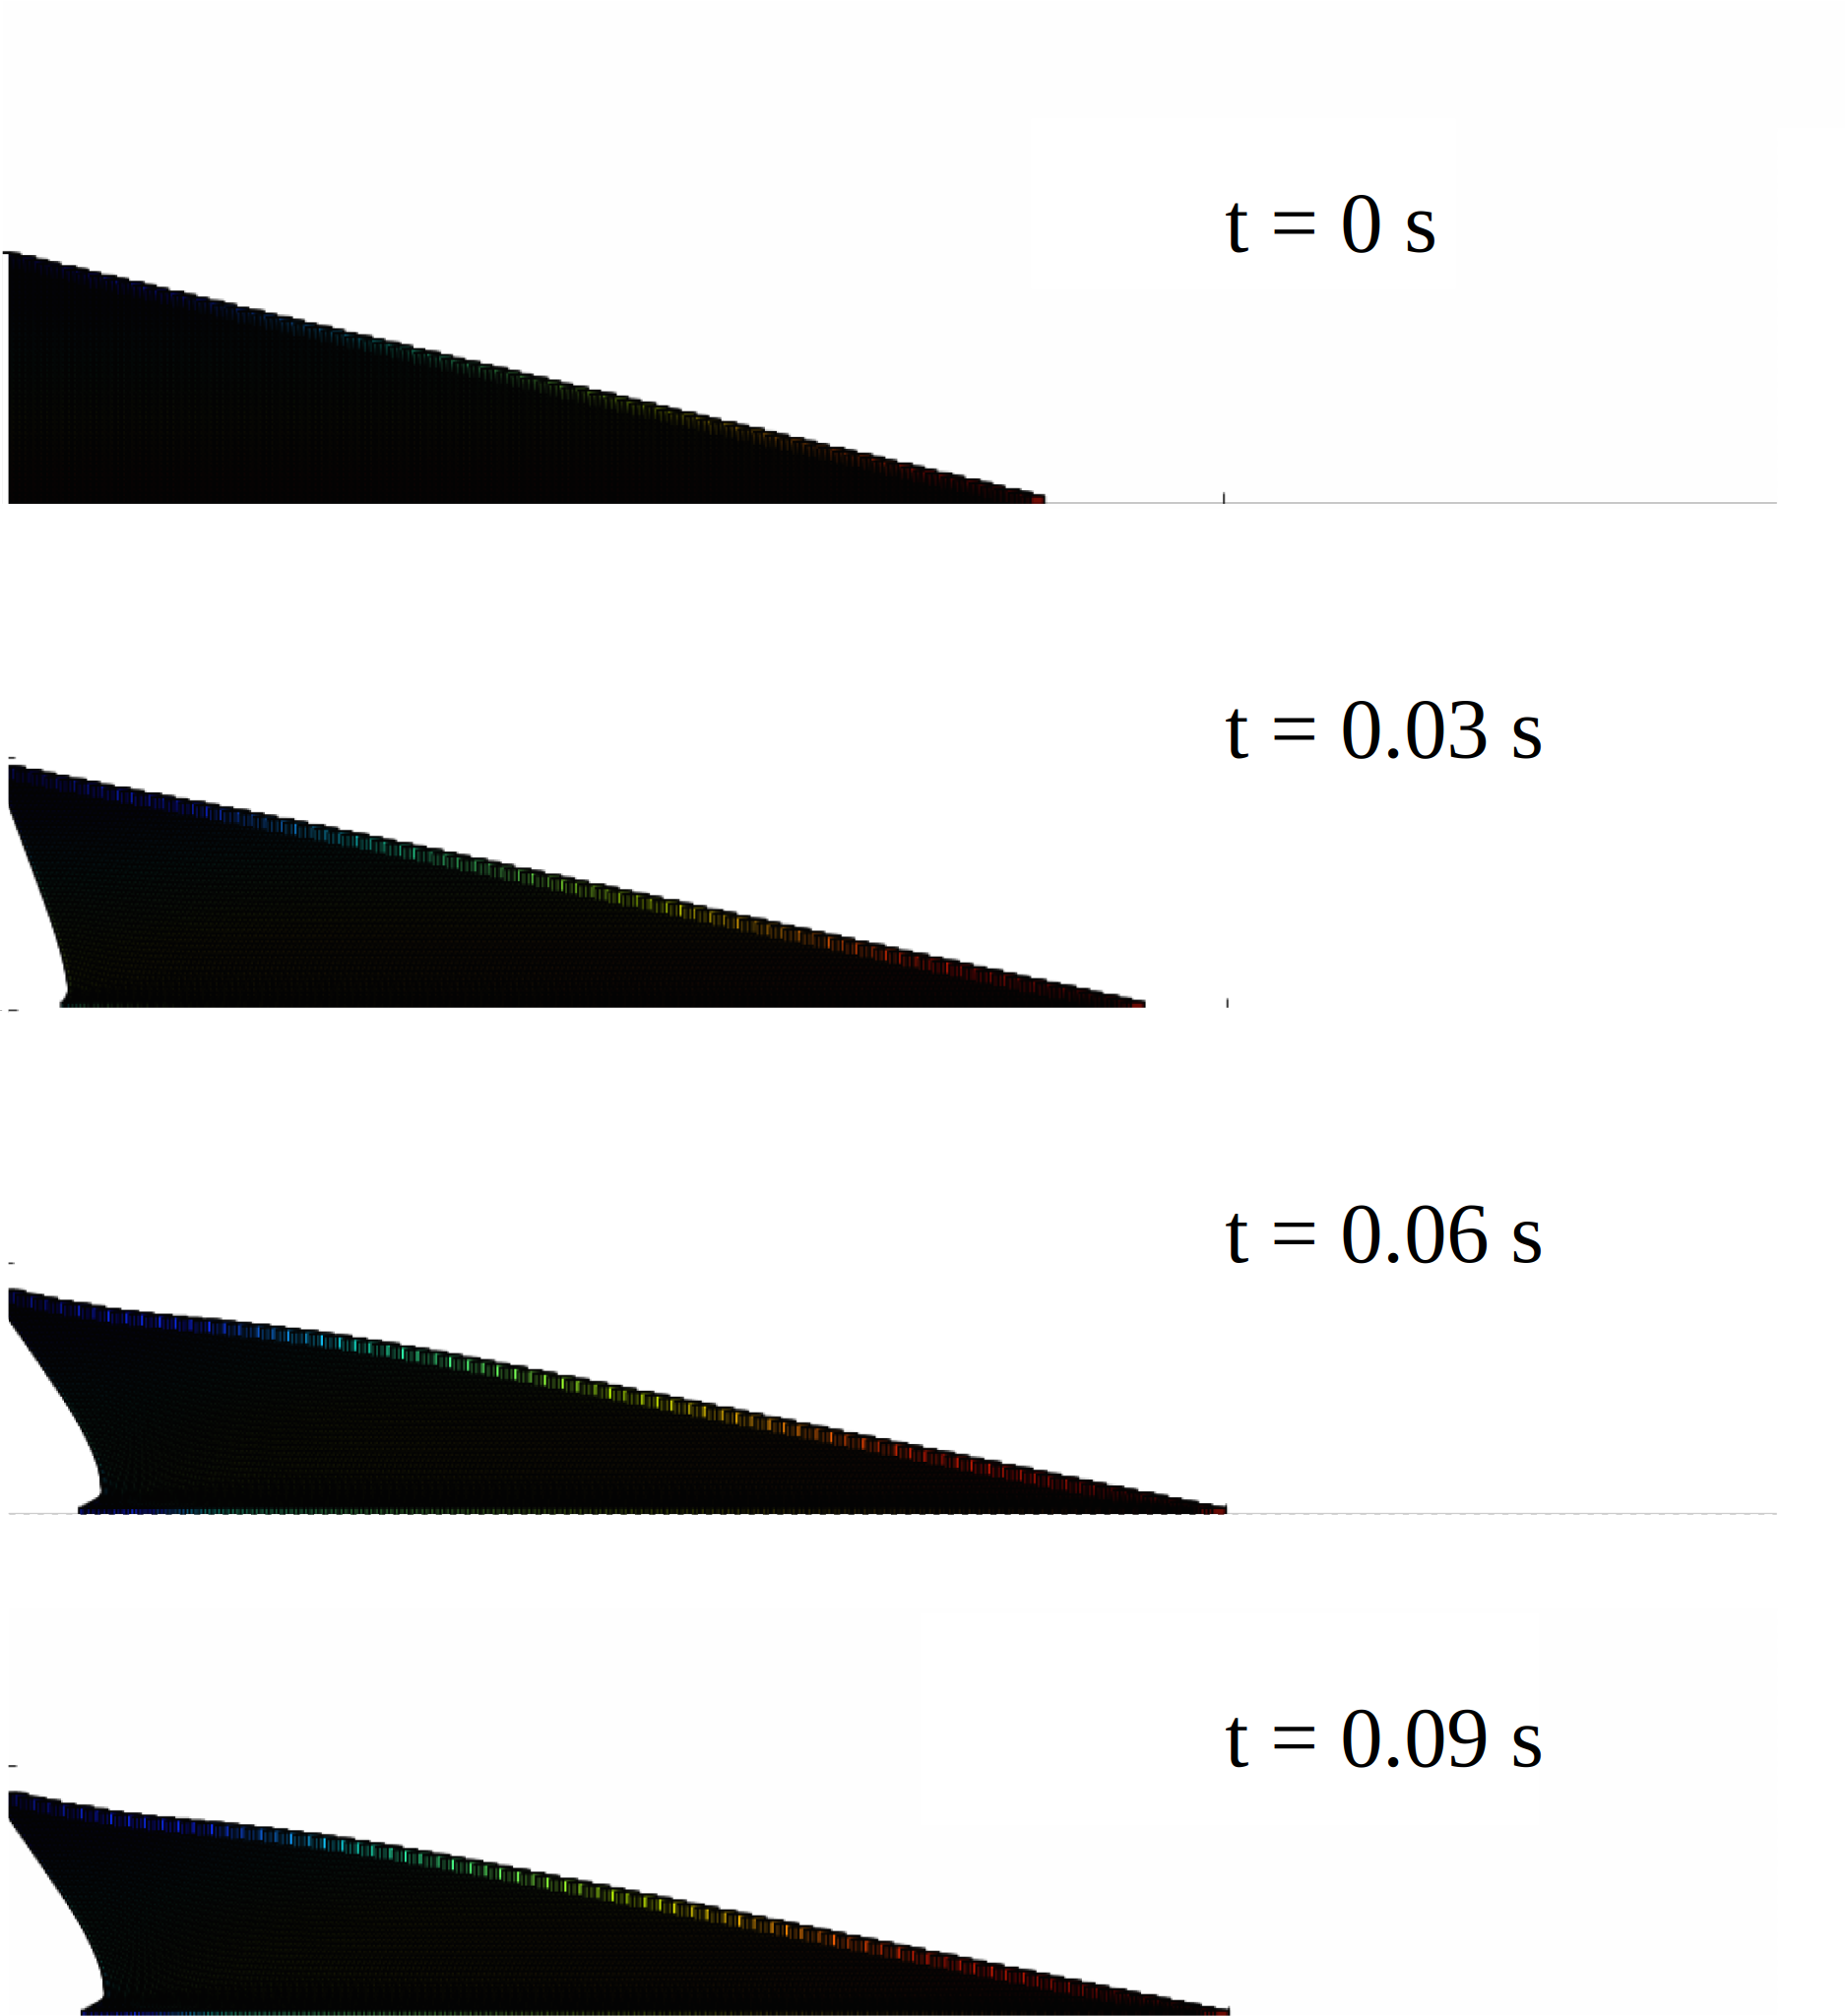
\includegraphics[width=\textwidth]{Gradient_Slope_Profile_200J}
\caption{MPM simulation of the initial stages of granular pile subjected to a 
gradient impact 
energy.}
\label{fig:Gradient_Slope_Profile_200J}
\end{figure}

\begin{figure}
\centering
\includegraphics[width=\textwidth]{Gradient_Slope_CD_200J}
\caption{CD simulation of the initial stages of granular pile subjected to a 
gradient impact 
energy.~\citep{Mutabaruka2013}.}
\label{fig:Gradient_Slope_CD_200J}
\end{figure}

The flow involves a transient with a sharp change in the geometry of the pile 
followed by continuous spreading. The gradient input energy applied to the 
granular slope mimics a horizontal quake from the bottom. Despite the creation 
of a cavity behind the flowing mass, the granular heap always remains in 
contact with the left wall irrespective of the input 
energy.~\Cref{fig:Runout_Eo_MPM_CD_DEM} shows the normalized run-out distance 
$(L_f - L_0)/L_0$ and total run-out time $t_f$ as a function of the input 
energy $E_0$. Two regimes characterized by power-law relationship between 
the run-out distance and time as a function of $E_0$ can be observed. In the 
first regime, corresponding to the range of low input energies $E_0 < 40 \ 
mgd$, the run-out distance observed varies as $L_f \propto (E_0)^\alpha$ with 
$\alpha 
\simeq 0.206 \pm 0.012$ over nearly one decade. Overall, the run-out distance 
predicted by the continuum approach matches the DEM simulations. At very low 
energies, DEM simulations show longer run-out distance due to local 
fluidisation. The difference in the run-out between DEM and CD arise mainly 
from the scales of description and the inelastic nature of Contact Dynamics. 
Similar behaviour between DEM and CD approaches was observed 
by~\citet{Radjai1997}. 


While the run-out exhibits a power-law relation with the initial input energy, 
DEM simulations show that the flow duration remains constant at a value  $t_f 
\simeq 60 \  (d/g)^{0.5}$ irrespective of the value of $E_0$. The constant 
run-out time, in grain-scale simulations, indicates the collapse of grain into 
the cavity left behind the pile. An average run-out speed can be defined as 
$v_s = (L_f - L_0) / t_f$. According to the data, $v_s \propto 
(E_0)^{0.52\pm 0.012}$. The error on the exponent represents the 
confidence interval of linear fits on the logarithmic scale. Since the initial 
average velocity varies as $v_0 \propto (E_0)^{0.5}$, this difference between 
the values of the exponents suggests that the mobilized mass during run-out 
declines when the input energy is increased.


\begin{figure}[tbph]
\centering
\begin{subfigure}[b]{0.975\textwidth}
\centering
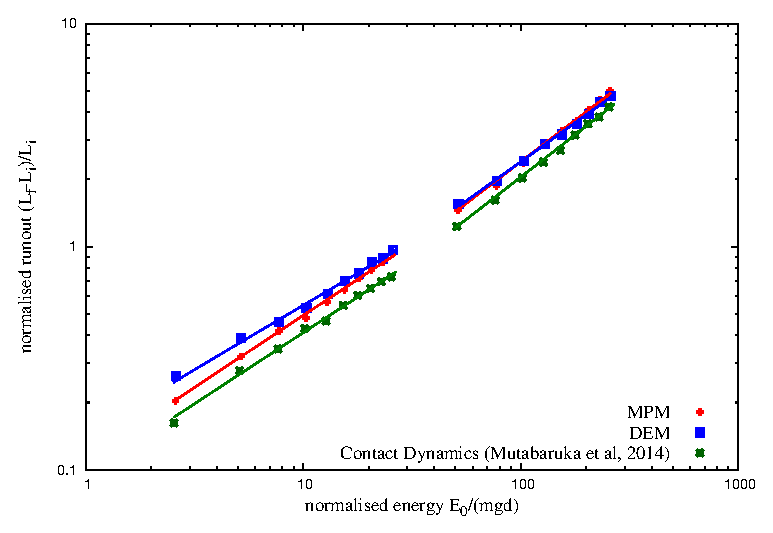
\includegraphics[width=\textwidth]{Runout_Eo_MPM_CD_DEM}
\caption{Run-out distance as a function of normalised input kinetic energy}
\label{fig:Runout_Eo_MPM_CD_DEM}
\end{subfigure}
\\
\begin{subfigure}[b]{0.975\textwidth}
\centering
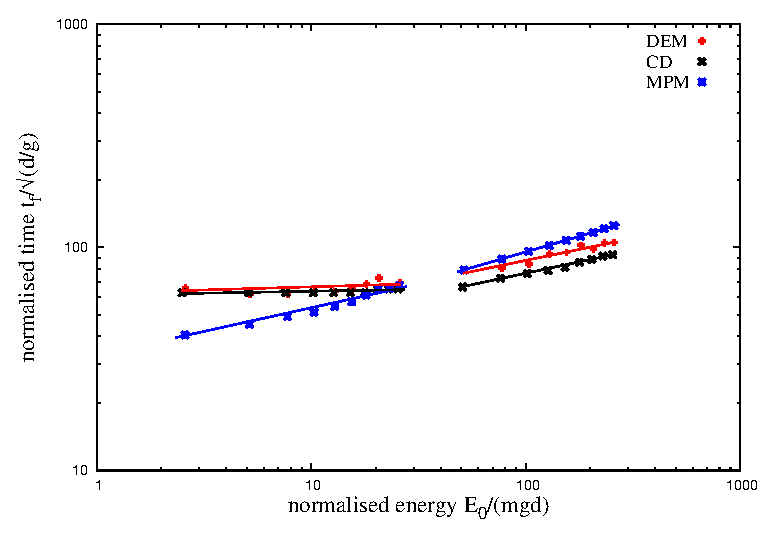
\includegraphics[width=\textwidth]{Tf_vs_Eo_Slope}
\caption{Duration of run-out as a function of normalised input kinetic energy}
\label{fig:Tf_vs_Eo_Slope}
\end{subfigure}
\caption{Run-out behaviour of a pile subjected a gradient impact energy}
\label{fig:Slope}
\end{figure}

In the second regime, corresponding to the range of high input energies  $E_0 > 
40 \ mgd$, the run-out distance varies as $L_f \propto (E_0)^{\alpha'}$ over 
one decade with $\alpha' \simeq 0.56\pm 0.04$ while the duration increases as 
$t_f \propto (E_0)^{\beta'}$ with $\beta' \simeq 0.33 \pm 0.02$. Hence, in this 
regime the average run-out speed varies as $v_s \propto (E_0)^{0.498 \pm 
0.01}$. This exponent is close to the value $0.5$ in $v_0 \propto (E_0)^{0.5}$, 
and hence, within the confidence interval of the exponents, in the second 
regime we may assume $\beta' \simeq \alpha' - 0.5$ and $v_s \propto v_0$. In 
the second regime, both DEM and MPM predict almost the same run-out behaviour. 
However, MPM predicts longer duration with increase in input energy.

It is worth noting that a similar power-law dependence of the run-out distance 
and time were found in the case of granular column collapse with respect to 
the initial aspect ratio. In the column geometry, the grains spread away 
owing to the kinetic energy acquired during gravitational collapse of the 
column.~\citet{Topin2012} found that the run-out distance varies as a power-law 
of the available peak kinetic energy at the end of the free-fall stage with an 
exponent $\simeq 0.5$. This value of exponent is lower than the run-out 
evolution observed in the second regime. This is, however, physically plausible 
since the distribution of particle kinetic energies at the end of the collapse 
is more chaotic than in this case where the energy is supplied from the very 
beginning in a well-defined shear mode. As pointed out by~\citet{Staron2005}, 
the distribution of kinetic energies is an essential factor for the run-out 
distance.

%-------------------------------------------------------------------------------------------
\subsection{Decay of kinetic energy}
\label{sec:decay}

The non-trivial evolution of the pile geometry in two regimes suggests that 
the energy supplied to the pile is not simply dissipated by shear and friction 
along the bottom plane. It is important to split the kinetic energy into the 
vertical and horizontal components ($K_{Ex}$ and $K_{Ey}$) of the velocity 
field. The input energy is in the $x$ component, but due to the creation 
of a cavity next  to the left wall and the rolling of the grains down the free 
surface of the pile and between grains, a fraction of the energy is first 
transferred to the vertical component of the velocity field and dissipated  
during the transient phase. The evolution of kinetic energy is studied to  
understand the behaviour of granular flow that is consistent with the evolution 
of pile shape.

The evolution of total kinetic energies $E_k$ with time for different values of 
the input energy $E_{ki}$ based on MPM simulations are shown in 
~\cref{fig:Energy_Time_Slope}. MPM simulations shows two distinct regimes in 
the normalised kinetic energy plot as a function of 
normalised time~\cref{fig:Normalised_Energy_Time_Slope}. However, DEM 
simulations (see~\cref{fig:Normalised_Energy_Time_Slope_DEM}) show that the 
energy evolution corresponding to low energy regime collapse nearly on to a 
single time evolution. This is consistent with the observation of run-out time 
$t_f$ independent of the input energy. In contrast, MPM simulations predict a 
power law relation between the run-out duration and input energy. However, the 
plots corresponding to high energy regime collapse only at the beginning of the 
run-out i.e. for $t < t_1 \simeq 7.5 \ (d/g)^{0.5}$. Although MPM simulations 
show higher duration of run-out (~\cref{fig:Energy_Time_Slope}), the total 
kinetic energy is completely dissipated at $t = 60 \sqrt{d/g}$. DEM simulations 
predict $t = 80 \sqrt{d/g}$ for the kinetic energy to be completely dissipated. 
This is due particle rearrangement at the free surface (~\cref{fig:voro_500}). 
The granular pile shows some dilation behaviour initially, which is due to 
grains rolling down to fill the cavity. 

\begin{figure}[tbhp]
\centering
\begin{subfigure}[b]{0.975\textwidth}
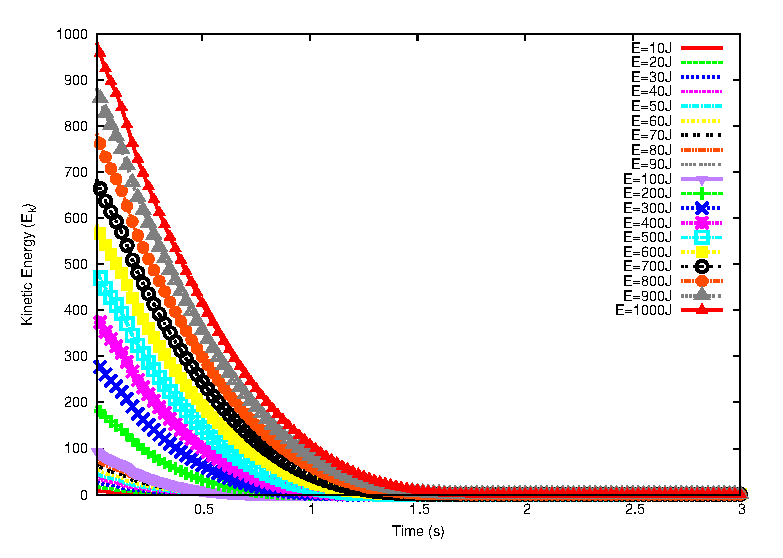
\includegraphics[width=\textwidth]{Energy_Slope}
\caption{Evolution of total kinetic energy with time}
\label{fig:energy_slope}
\end{subfigure}
\\
\begin{subfigure}[b]{0.975\textwidth}
\centering
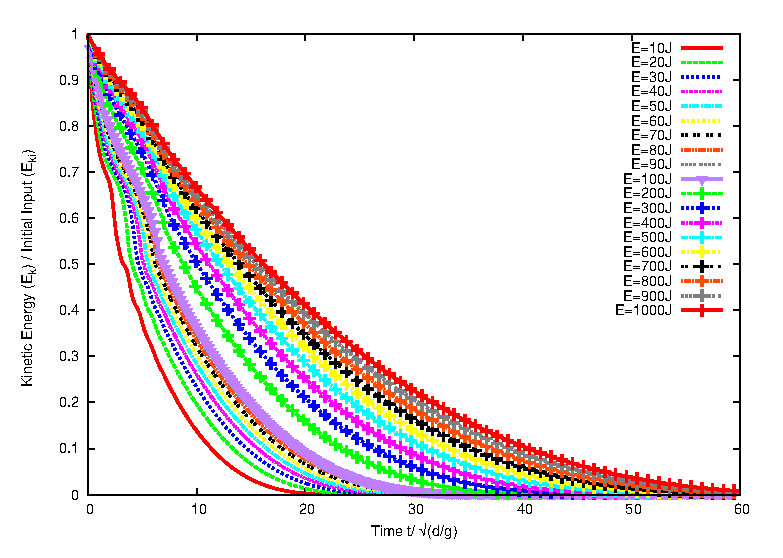
\includegraphics[width=\textwidth]{Normalised_Energy_Time_Slope}
\caption{Evolution of normalised kinetic energy with normalised time}
\label{fig:Normalised_Energy_Time_Slope}
\end{subfigure}
\caption{Evolution of kinetic energy with time (MPM)}
\label{fig:Energy_Time_Slope}
\end{figure}

\begin{figure}[tbhp]
\centering
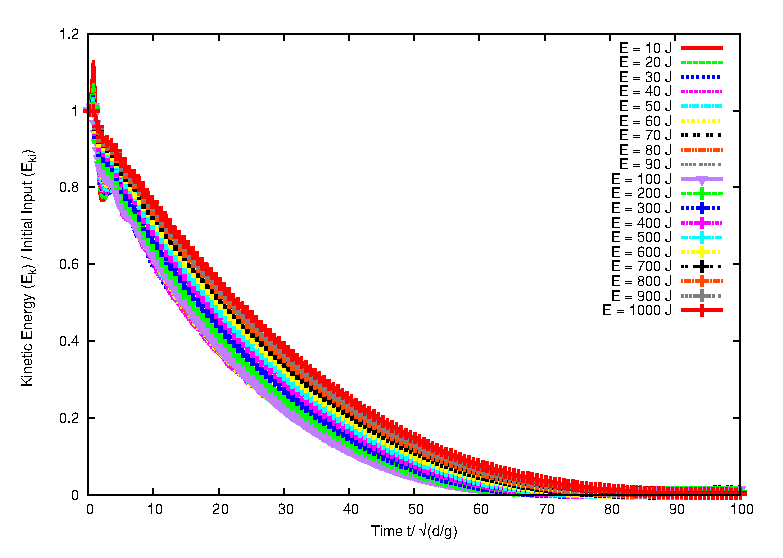
\includegraphics[width=0.9\textwidth]{Normalised_Energy_Time_Slope_DEM}
\caption{Evolution of normalised kinetic energy with normalised time}
\label{fig:Normalised_Energy_Time_Slope_DEM}
\end{figure}

\begin{figure}[tbhp]
\centering
\includegraphics[width=0.9\textwidth]{voro_500}
\caption{Evolution of packing density with time $E_0 = 152 mgd$ (DEM)}
\label{fig:voro_500}
\end{figure}

~\Cref{fig:Normalised_KEx_KEy_Slope} displays the evolution of kinetic energy 
in the translational ($E_x$ and $E_y$) degrees of freedom. $E_x$ decays similar 
to the total energy dissipation, but $E_y$ increases and passes through a peak 
before decaying rapidly to a negligible level. The transient is best 
observed for $E_y$, which has significant values only for $t< t_1$. This energy 
represents the proportion of kinetic energy transferred to the $y$ component of 
the velocity field  due to the destabilization of the pile and collapse of 
grains in the cavity behind the pile. Higher proportion of vertical 
acceleration $E_{ky}/E_0$ is observed for lower values of input energy $E_0$. 
This means that, at lower input energies a larger fraction of the energy is 
consumed in the destabilization process. Whereas at a higher input energies, 
most of the energy is dissipated in the spreading phase. For this reason, the 
total duration $t_1$ of this destabilization phase is nearly the same in 
both regimes and its value is controlled by the gravity rather than the input 
energy. The height of the pile being of the order of $80 \ d$, the total 
free-fall time for a particle located at this height is $\simeq 12 \ 
(d/g)^{0.5}$, which is of the same order as $t_1$. The contribution of the  
rotational energy during the transient stage and the spreading stage is 
negligible. 

\begin{figure}[tbhp]
\centering
\begin{subfigure}[b]{0.975\textwidth}
\includegraphics[width=\textwidth]{Normalised_KEx_Slope}
\caption{Evolution of normalised horizontal kinetic energy with time}
\label{fig:Normalised_KEx_Slope}
\end{subfigure}
\\
\begin{subfigure}[b]{0.975\textwidth}
\centering
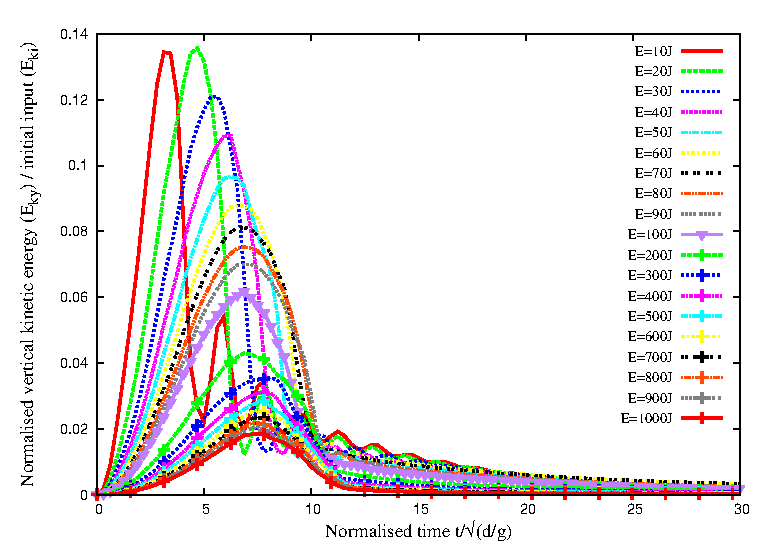
\includegraphics[width=\textwidth]{Normalised_KEy_Slope}
\caption{Evolution of normalised vertical kinetic energy with time}
\label{fig:Normalised_KEy_Slope}
\end{subfigure}
\caption{Evolution of vertical and horizontal kinetic energy with time (MPM)}
\label{fig:Normalised_KEx_KEy_Slope}
\end{figure}

To analyse the second phase for higher input energies, the 
kinetic energy $E'_{kx0}$ available at the end of the transient phase is 
considered. This energy is responsible for most of the run-out and hence it is 
expected to 
control the run-out distance and time.~\Cref{fig:Normalised_KExExop_Slope} 
shows the evolution of $E_{kx}$ normalized by $E'_{kx0}$ as a function of time. 
The plots have seemingly the same aspect but they show different decay times. A 
decay time $\tau$ can be defined as the time required for $E_{kx}$ to decline 
by a factor $1/2$.~\Cref{fig:ExEx0_vs_ttau} shows the same data in 
which the time $t'$ elapsed since $t_1$ is normalized by $\tau$. Interestingly, 
now all the data nicely collapse on to a single curve. However, this curve can 
not be fitted by simple functional forms such as variants of exponential decay. 
This means that the spreading of the pile is not a self-similar process in 
agreement with the fact that the energy fades away in a finite time $t'_f$. 

\begin{figure}[tbhp]
\centering
\includegraphics[width=\textwidth]{Normalised_KExExop_Slope}
\caption{Evolution of kinetic energy in the $x$ component of the
velocity field normalized by the available kinetic energy at the
end of the transient as a function of time elapsed since the
same instant (MPM).}
\label{fig:Normalised_KExExop_Slope}
\end{figure}

\begin{figure}[tbhp]
\centering
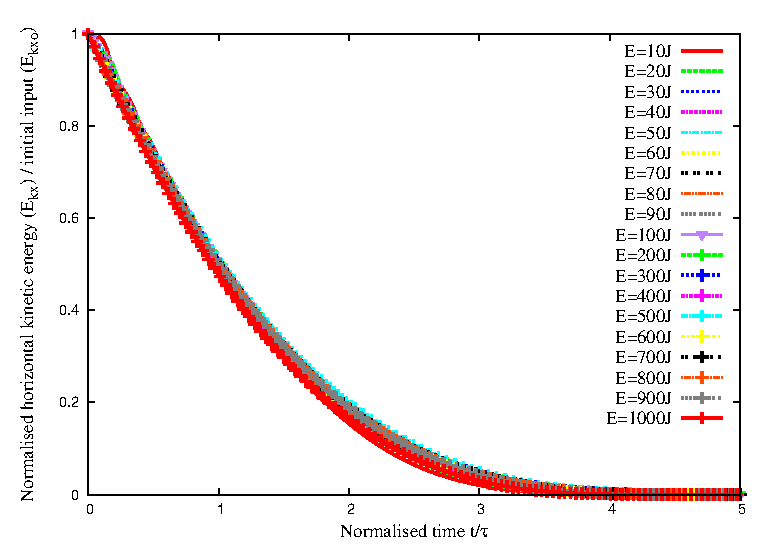
\includegraphics[width=\textwidth]{EkxKoTTau_Slope}
\caption{Evolution of kinetic energy in the $x$ component of 
the velocity field  normalized by the available kinetic energy at the end of 
the transient as a function of normalized time (MPM).}
\label{fig:ExEx0_vs_ttau}
\end{figure}


The scaling of the data with the decay time $\tau$ suggests that the 
run-out time $t'_f$, since the beginning of the second phase, might be a simple 
function of $\tau$.~\Cref{fig:tp_tau_mgd} shows both $t'_f$ and $\tau$ as 
a function of $E'_{x0}$, where a power-law relation can be observed for both 
time scales. The run-out time $t'_f \propto (E'_{x0})^{\beta'}$ has the 
same exponent $\beta' \simeq 0.33 \pm 0.02$ as $t_f$ as a function of $E_0$. 
For the decay time we have $\tau \propto (E'_{x0})^{\beta''}$ with $\beta'' 
\simeq 0.38 \pm 0.03$. The relation between the two times can thus be expressed 
as (see~\cref{fig:tpTau})
\begin{equation}
t'_f = k  \ \tau \, (E'_{x0})^{\beta'' - \beta'} \,,
\label{eqn:t'f}
\end{equation}
where $k \simeq 5 \pm 0.4$ and $\beta'' - \beta' \simeq -0.06 \pm 0.05$. This 
value is small enough to be neglected within the confidence interval of the 
data. It is therefore plausible to assume that the run-out time is a multiple 
of the decay time and the spreading process is controlled by a single time. A 
weak dependence on the energy $E'_{kx0}$ is consistent with the fact that the  
energy available at the beginning of the second phase is not dissipated in the 
spreading process (calculated from the position of the tip of the pile) since  
the pile keeps deforming by the movements of the grains at the free surface 
even when the tip comes to rest. This can explain the small difference between 
the two exponents as observed here.


\begin{figure}[tbhp]
\centering
\begin{subfigure}[b]{0.975\textwidth}
\includegraphics[width=\textwidth]{tp_tau_mgd}
\caption{Power law evolution of $t'_f$ and $\tau$ as a function of kinetic 
energy $E'_{kx0}$.}
\label{fig:tp_tau_mgd}
\end{subfigure}
\\
\begin{subfigure}[b]{0.975\textwidth}
\centering
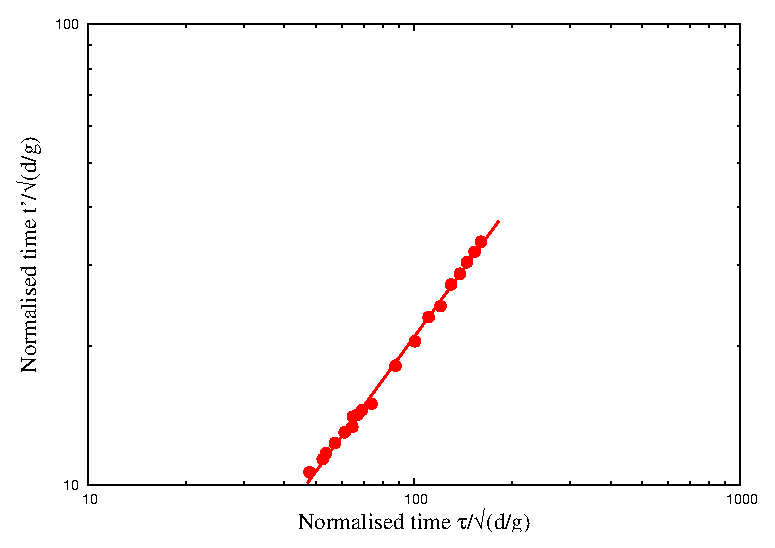
\includegraphics[width=\textwidth]{tpTau}
\caption{Linear relationship between decay time and run-out time after the 
transient as a function of the normalised kinetic energy $E_{kx0}$.}
\label{fig:tpTau}
\end{subfigure}
\caption{Decay time and run-out time as a function of the normalised kinetic 
energy $E_{kx0}$.}
\label{fig:tp_Tau}
\end{figure}


%-------------------------------------------------------------------------------
\subsection{Effect of friction}
\label{sec:parameters}

The run-out distance, duration of flow, and the dissipation of kinetic energy 
are controlled by the input energy and collective dynamics of the whole pile. 
However, the run-out behaviour is expected to also depend on the base friction. 
A series of simulations with different values of base friction was performed 
using MPM to analyse the influence of friction on the run-out behaviour. The 
influence of friction on the run-out behaviour is shown in
~\cref{fig:runout_fric_slope}. The exponent of the 
power-law relation between the run-out and input energy has a weak dependence 
on the base friction, the proportionality constant, however, is affected by the 
change in the base friction. This behaviour is similar to that observed in 
granular column collapse with varying initial 
properties~\citep{Balmforth2005,Lajeunesse2005}. 

CD simulations using different values of coefficient of restitution shows no 
difference in the run-out behaviour. At large input energies, the pile remains 
in a dense state so that multiple collisions inside the pile occur at small 
time scales compared to the deformation time. When the restitution coefficients 
are increased, more collisions occur during a longer time interval but the 
overall energy dissipation rate by collisions remains the same. This effect is 
a seminal example of collective effects which erase the influence of local 
parameters at the macroscopic scale.

In contrast with the restitution coefficients, the effect of friction 
coefficient, however, is quite important for the run-out. MPM simulations with 
varying friction coefficient shows that, both the run-out distance and the 
decay time decrease as the friction coefficient is increased. This 
effect is much more pronounced at low values of the friction coefficient. 
Similar behaviour was observed in CD simulations. The run-out time, for 
example, is reduced by a factor of $\approx 4$ as $\mu_s$ is increased from 0.1 
to 0.2 while the change in the run-out and duration is less effected with 
increase in friction coefficient. This ``saturation effect" 
can be observed in a systematic way in simple shear tests. The dissipation rate 
may reach a saturation point where the dilation of granular materials and 
rolling of the grains change in response to increase in friction coefficient 
\cite{Estrada2008}.

\begin{figure}[tbhp]
\centering
\begin{subfigure}[b]{0.95\textwidth}
\centering
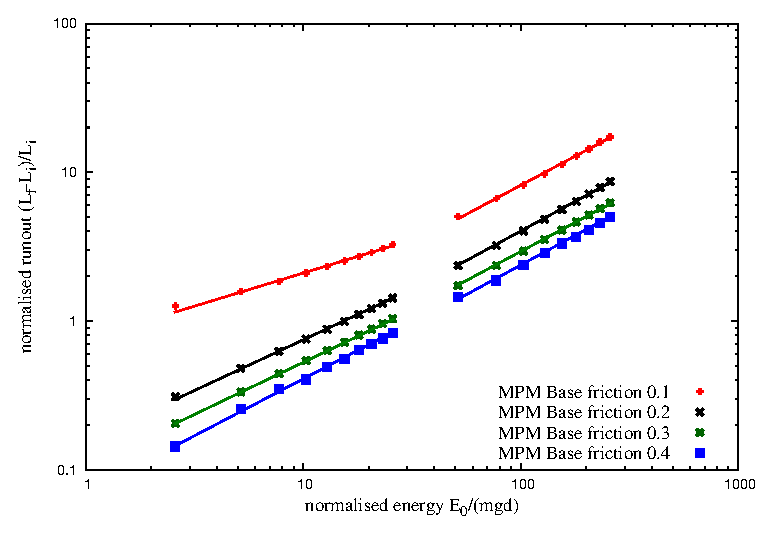
\includegraphics[width=\textwidth]{runout_fric_slope}
\caption{Effect of friction on the run-out distance}
\label{fig:runout_fric_slope}
\end{subfigure}
\\
\begin{subfigure}[b]{0.95\textwidth}
\centering
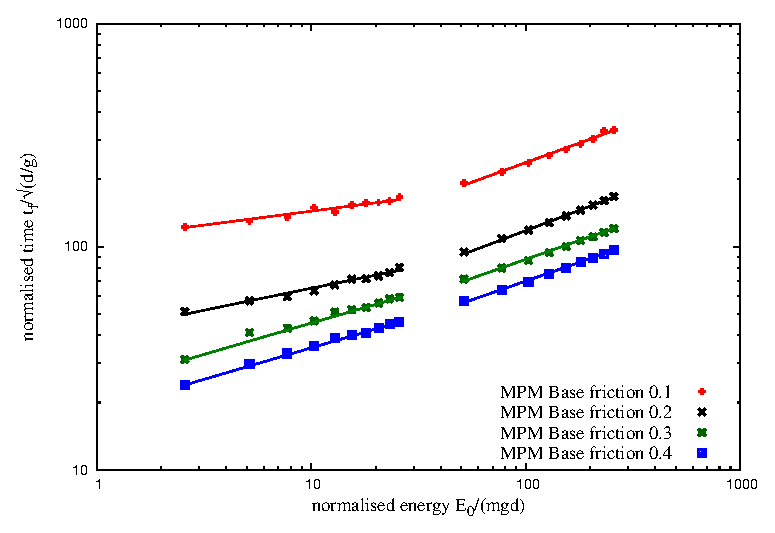
\includegraphics[width=\textwidth]{time_fric_slope}
\caption{Effect of friction on the duration of run-out.}
\label{fig:time_fric_slope}
\end{subfigure}
\caption{Effect of friction on the run-out behaviour}
\label{fig:fric_slope}
\end{figure}

%-------------------------------------------------------------------------------

\subsection*{Effect kinetic energy distribution}

~\citet{Staron2005} observed that the distribution of kinetic energies is an 
essential factor for the run-out distance. In order to understand the influence 
of energy distribution on the run-out behaviour, granular pile subjected to two 
different velocity fields was studied. A uniform velocity $V_{xo} (y) = V_0$ is 
applied to the entire pile, in contrast to the gradient impact velocity. 
Snapshots of flow kinematics at initial stages are shown 
in~\cref{fig:Uniform_Slope_Profile_200J} (MPM simulations) 
and~\cref{fig:Uniform_Slope_DEM_200J} (DEM). It can be observed from the 
figures that the continuum behaviour is identical to that of grain-scale 
simulations. As each grain experiences the same velocity, grains located at the 
top of the slope are pushed farther away and unlike the gradient input 
velocity, the cavity left behind the granular mass is not filled by the soil 
grains at the top. 
\begin{figure}[tbph]
\centering
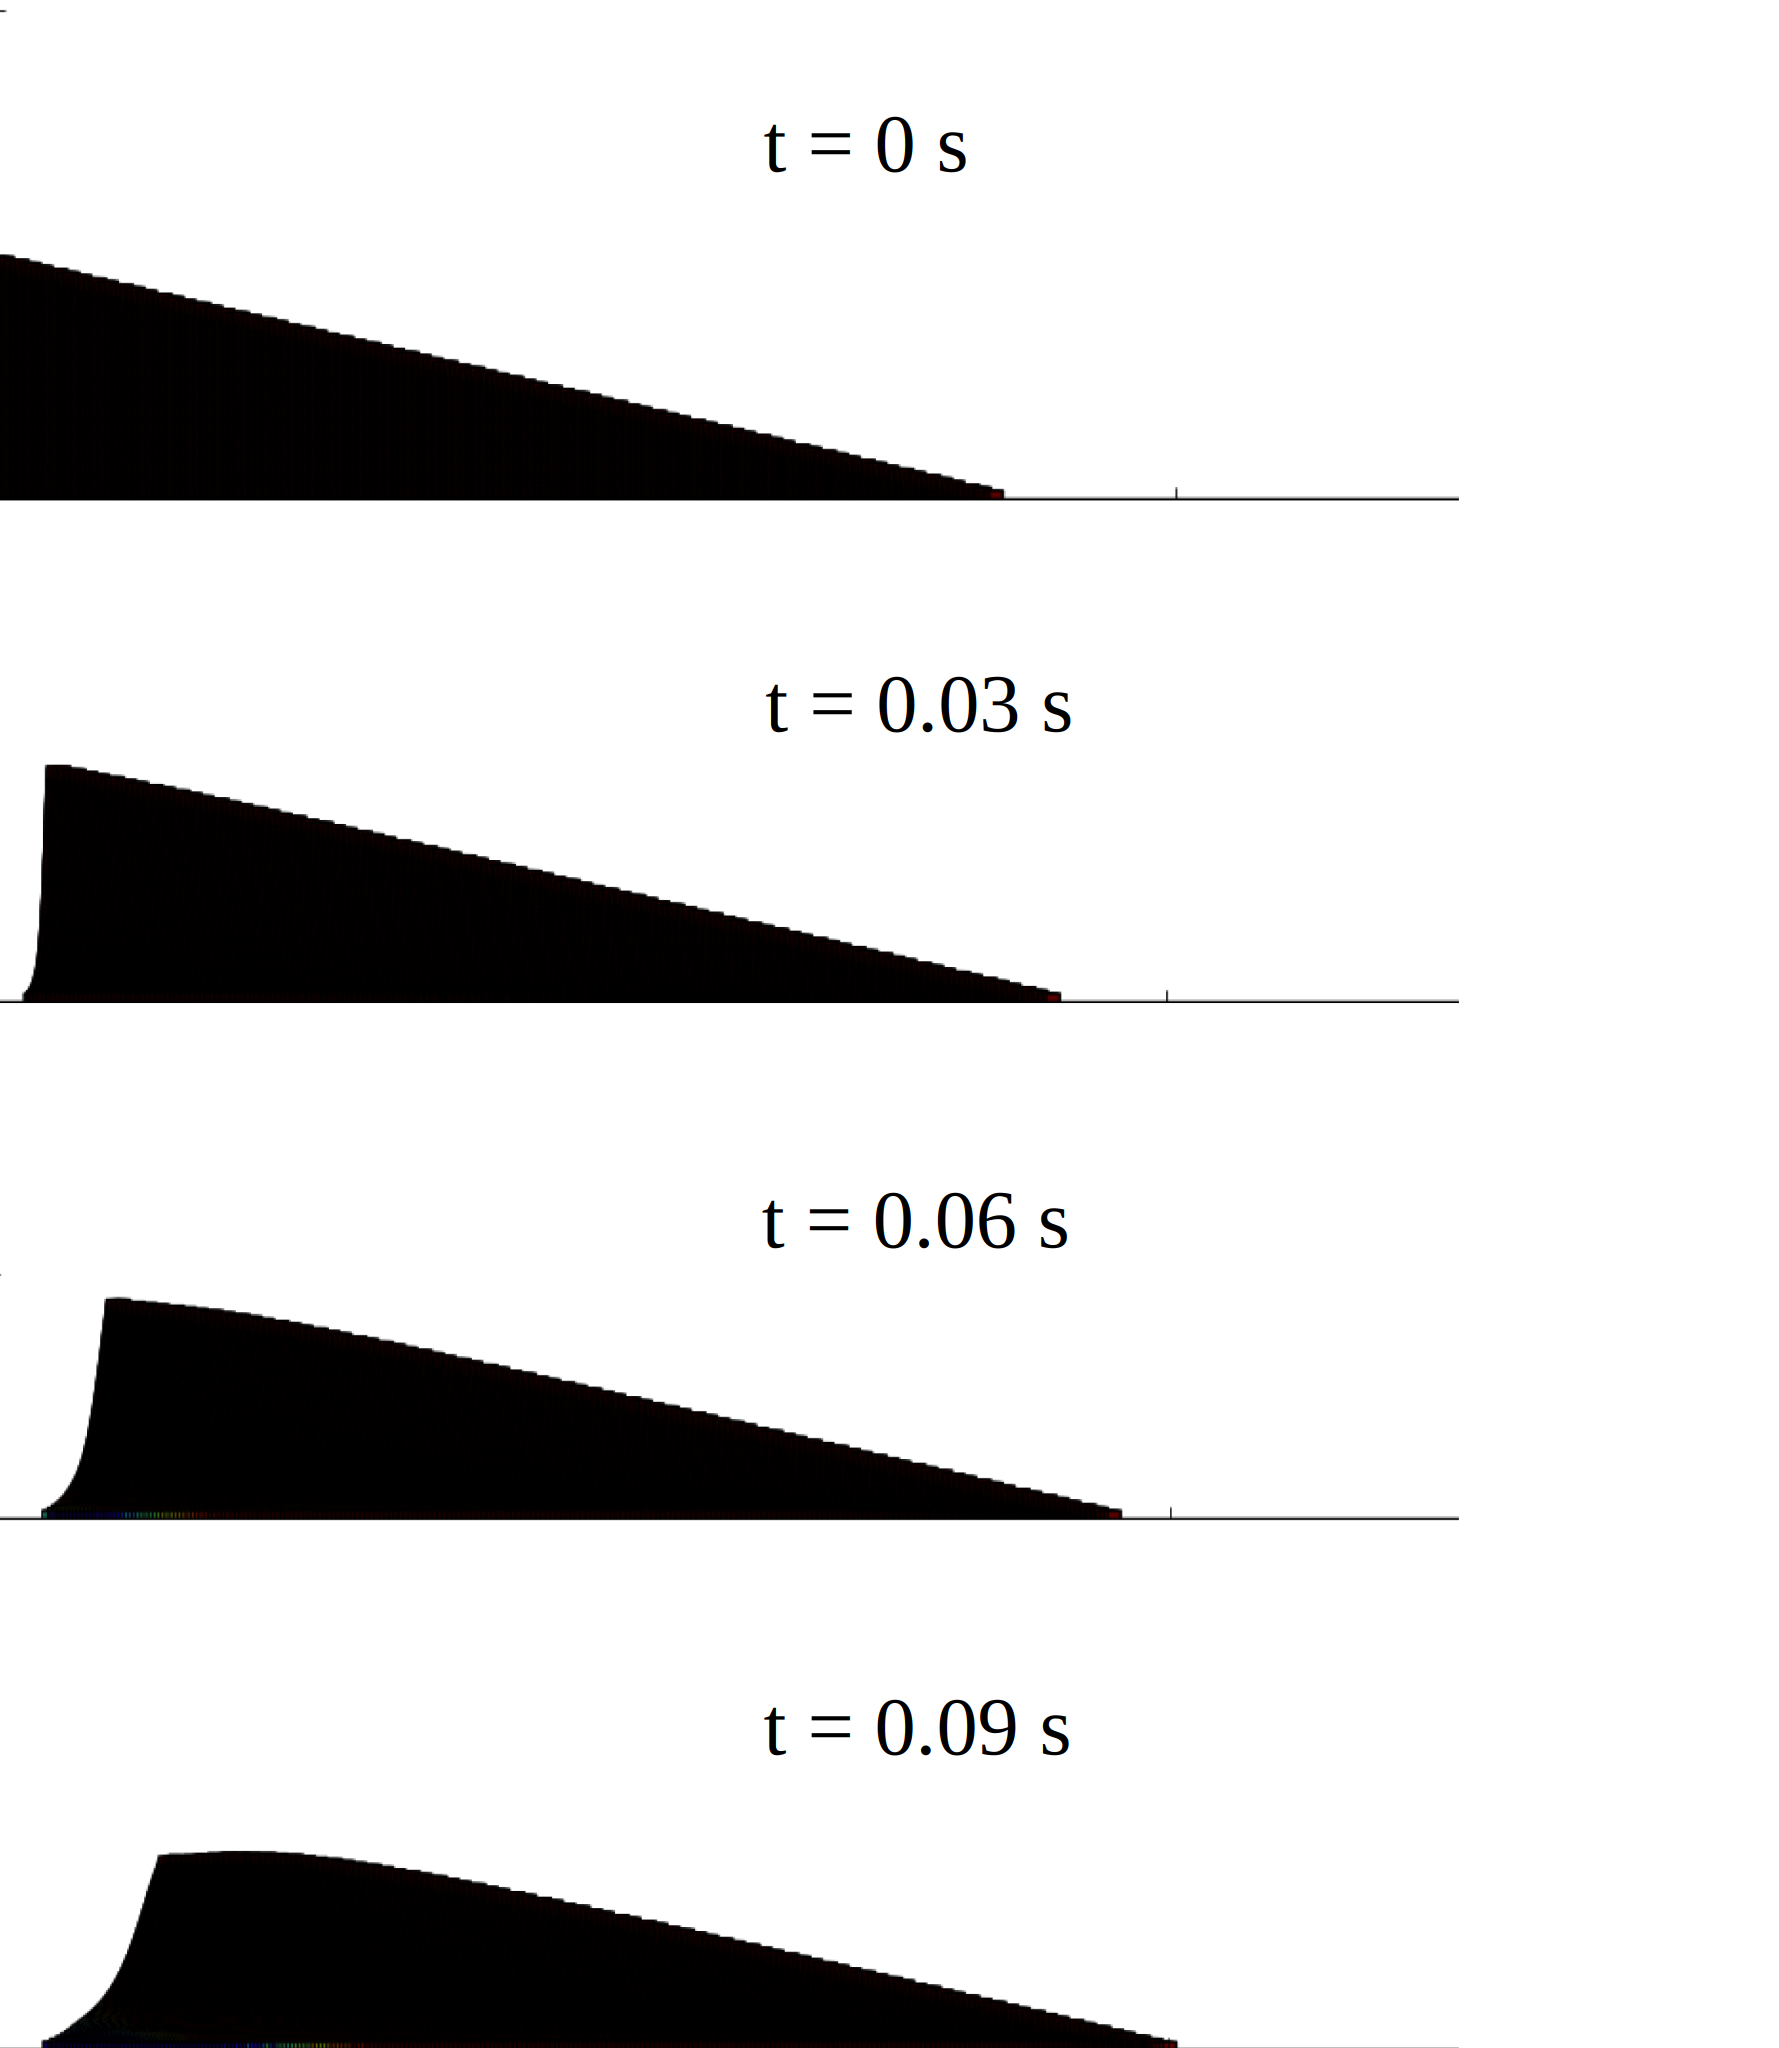
\includegraphics[width=\textwidth]{Uniform_Slope_Profile_200J}
\caption{Snapshots of MPM simulations of the evolution of granular pile 
subjected to a gradient impact energy $E_0 = 61 \ mgd$.}
\label{fig:Uniform_Slope_Profile_200J}
\end{figure}

\begin{figure}[tbph]
\centering
\includegraphics[width=\textwidth]{Uniform_Slope_DEM_200J}
\caption{Snapshots of DEM simulations of the evolution of granular pile 
subjected to a gradient impact energy $E_0 = 61 \ mgd$.}
\label{fig:Uniform_Slope_DEM_200J}
\end{figure}

~\Cref{fig:Runout_Eo_GU} shows the influence of velocity distribution on the 
run-out behaviour. At low input energy, the gradient velocity distribution 
shows significanly longer run-out in comparison to uniform velocity 
distribution.~\Cref{sec:decay} showed that at lower input energies a larger 
fraction of the energy is consumed in the destabilization process. Which means 
that the amount energy available for flow is less, in uniform velocity 
distribution, this energy is even smaller due to the uniform distribution of 
the initial impact velocity. However at higher input energy, where most of the 
energy is dissipated during the spreading phase, the run-out distance has a 
weak dependence on the distribution of velocity in the granular mass. The 
duration of the flow shows similar behaviour to the run-out, however, the slope 
subjected a gradient velocity flows quicker than the uniform velocity 
distribution. Gradient velocity distribution provides more input energy at the 
initial stage to overcome the frictional resistance at the base. Hence, it can 
be observed that the material property and the distribution of kinetic energy 
in the system has a non-trivial influence on the flow kinematics and the 
internal flow structure.

\begin{figure}[tbph]
\centering
\begin{subfigure}[b]{0.95\textwidth}
\centering
\includegraphics[width=\textwidth]{Runout_Eo_GU}
\caption{Run-out distance as a function of normalised input kinetic energy}
\label{fig:Runout_Eo_GU}
\end{subfigure}
\\
\begin{subfigure}[b]{0.95\textwidth}
\centering
\includegraphics[width=\textwidth]{time_Eo_GU}
\caption{Duration of run-out as a function of normalised input kinetic energy}
\label{fig:time_Eo_GU}
\end{subfigure}
\caption{Effect of input velocity distribution on the run-out behaviour}
\label{fig:GU}
\end{figure}
%-------------------------------------------------------------------------------

\subsection{Effect of mesh size and number of material points per cell}
\label{sec:MPM_points_per_cell}

\citet{Abe2013} and \citet{Coetzee2005} observed influence of number of 
material points per cell and mesh size effect on the numerical simulations.

\begin{figure}[tbhp]
\centering
\begin{subfigure}[b]{0.95\textwidth}
\includegraphics[width=\textwidth]{Runout_50}
\caption{$E_0=12.7mgd$}
\label{fig:Runout_50}
\end{subfigure}
\\
\begin{subfigure}[b]{0.95\textwidth}
\centering
\includegraphics[width=\textwidth]{Runout_500}
\caption{$E_0=152mgd$}
\label{fig:Runout_500}
\end{subfigure}
\caption{Evolution of run-out with time for varying material points per cell.}
\label{fig:Runout_MPM}
\end{figure}


\begin{figure}[tbhp]
\centering
\begin{subfigure}[b]{0.95\textwidth}
\includegraphics[width=\textwidth]{KE_50}
\caption{$E_0=12.7mgd$.}
\label{fig:KE_50}
\end{subfigure}
\\
\begin{subfigure}[b]{0.95\textwidth}
\centering
\includegraphics[width=\textwidth]{KE_500}
\caption{$E_0=152mgd$}
\label{fig:KE_500}
\end{subfigure}
\caption{Evolution of kinetic with time for varying material points per cell}
\label{fig:KE_MPM}
\end{figure}

\begin{figure}[tbhp]
\centering
\begin{subfigure}[b]{0.95\textwidth}
\includegraphics[width=\textwidth]{50}
\caption{$E_0=12.7mgd$.}
\label{fig:50}
\end{subfigure}
\\
\begin{subfigure}[b]{0.95\textwidth}
\centering
\includegraphics[width=\textwidth]{500}
\caption{$E_0=152mgd$.}
\label{fig:500}
\end{subfigure}
\caption{Evolution of run-out and duration of flow  for varying material points 
per cell.}
\label{fig:MPM_Size_Effect}
\end{figure}


\begin{figure}[tbhp]
\centering
\includegraphics[height=\textheight]{MPM_50ppc}
\caption{Effect of number of material points on cell on the run-out behaviour 
$E_0=12.7mgd$. 
Velocity profile (\si{\m\per\s}) of granular pile subjected to gradient impact 
loading.}
\label{fig:MPM_50ppc}
\end{figure}


\begin{figure}[tbhp]
\centering
\includegraphics[height=\textheight]{MPM_500ppc}
\caption{Effect of number of material points on cell on the run-out behaviour 
$E_0=152mgd$. 
Velocity profile (\si{\m\per\s}) of granular pile subjected to gradient impact 
loading.}
\label{fig:MPM_500ppc}
\end{figure}

\subsection{Comparison with granular column collapse}


\begin{figure}[tbhp]
\centering
\includegraphics[width=0.95\textwidth]{Slope_Column}
\caption{Comparison of column collapse with slope subjected to impact loading.}
\label{fig:Slope_Column}
\end{figure}

\section{Summary}
Multi-scale simulation of granular column collapse was performed to understand 
the ability and limitations of continuum models to capture the micro-mechanics 
of dense granular flows. The run-out behaviour predicted by both continuum and 
DEM simulations matches for columns with small aspect ratios, where the 
dissipation is predominantly frictional. However, MPM predicts longer run-out 
distance for columns with higher aspect ratios. Energy evolution studies using 
DEM simulations reveal that the run-out behaviour is independent of frictional 
properties of the granular material and collision predominates the initial 
free-fall regime. The lack of a collisional energy dissipation mechanism in MPM 
results in over prediction of run-out distances. 


The choice of this geometry was motivated by our main goal  to focus on the 
effect of an input energy on the consecutive dynamics of a granular material.
For the range of input energies investigated in this pushing test by means of 
contact dynamics simulations, we observed a power-law dependence of the 
run-out distance and time with non-trivial exponents. This is a central result 
of this work as it reveals that the power-law behaviour is a generic feature of 
granular dynamics. The values of the exponents are not simple functions of 
the geometry. 

We also evidenced two regimes with different values of the exponents: 
a low-energy regime and a high-energy regime. The first regime  
reflects mainly the destabilization of the pile by the quake with a run-out 
time 
independent of the input energy whereas the second regime is governed by the 
spreading dynamics induced by the higher value of the input energy. We showed 
that the evolution of the pile in this high-energy regime can be described by a 
characteristic decay time and the energy available at the end of the first 
stage where the pile is destabilized by the quake. 

This work may be pursued along two directions: 1) experimental 
realization of a similar setup with different modes of energy injection and 
2) investigating the effect of various particle shapes or the presence of an 
ambient fluid. Although numerical simulations are generally reliable 
with realistic results found in the past studies of steady flows, we believe 
that the transients are more sensitive situations than steady states and the  
experiments are necessary for checking the validation of the results suggested 
by the simulations. Provided a convenient method is used for supplying kinetic 
energy homogeneously into a pile, our configuration is also interesting for 
the investigation of the behavior of a pile immersed in a viscous 
fluid.
